\documentclass[10pt,a4paper]{article}
\usepackage[UTF8,fontset = windows]{ctex}
\setCJKmainfont[BoldFont=黑体,ItalicFont=楷体]{华文中宋}
\usepackage{amssymb,amsmath,amsfonts,amsthm,mathrsfs,dsfont,graphicx}
\usepackage{ifthen,indentfirst,enumerate,color,titletoc}
\usepackage{tikz}
\usepackage{makecell}
\usepackage{longtable}
%\usepackage{mathptmx}

\usetikzlibrary{arrows,calc,intersections,patterns,decorations.pathreplacing,angles}
\usepackage[bf,small,indentafter,pagestyles]{titlesec}
\usepackage[top=1in, bottom=1in,left=0.8in,right=0.8in]{geometry}
\renewcommand{\baselinestretch}{1.65}
\newtheorem{defi}{定义~}
\newtheorem{eg}{例~}
\newtheorem{ex}{~}
\newtheorem{rem}{注~}
\newtheorem{thm}{定理~}
\newtheorem{coro}{推论~}
\newtheorem{axiom}{公理~}
\newtheorem{prop}{性质~}
\newcommand{\blank}[1]{\underline{\hbox to #1pt{}}}
\newcommand{\bracket}[1]{(\hbox to #1pt{})}
\newcommand{\onech}[4]{\par\begin{tabular}{p{.9\textwidth}}
A.~#1\\
B.~#2\\
C.~#3\\
D.~#4
\end{tabular}}
\newcommand{\twoch}[4]{\par\begin{tabular}{p{.46\textwidth}p{.46\textwidth}}
A.~#1& B.~#2\\
C.~#3& D.~#4
\end{tabular}}
\newcommand{\vartwoch}[4]{\par\begin{tabular}{p{.46\textwidth}p{.46\textwidth}}
(1)~#1& (2)~#2\\
(3)~#3& (4)~#4
\end{tabular}}
\newcommand{\fourch}[4]{\par\begin{tabular}{p{.23\textwidth}p{.23\textwidth}p{.23\textwidth}p{.23\textwidth}}
A.~#1 &B.~#2& C.~#3& D.~#4
\end{tabular}}
\newcommand{\varfourch}[4]{\par\begin{tabular}{p{.23\textwidth}p{.23\textwidth}p{.23\textwidth}p{.23\textwidth}}
(1)~#1 &(2)~#2& (3)~#3& (4)~#4
\end{tabular}}
\begin{document}
\begin{enumerate}[1.]


\item 例1  求$\theta$, 使复数$z=\cos 2\theta +(\tan ^2\theta -\tan \theta -2)i$是:
(1)实数.			(2)纯虚数.			(3)零.
解  (1)由$\tan ^2\theta -\tan \theta -2=0$, 得$\tan \theta =-1$, $\tan \theta =2$,
∴$\theta =k\pi -\dfrac{\pi }4$, $\theta =k\pi +\arctan 2$($k\in \mathbf{Z}$).
(2)由$\begin{cases} \cos 2\theta =0, \\ (\tan \theta -2)(\tan \theta +1)\ne 0, \end{cases}$得$\begin{cases} \cos ^2\theta -\sin ^2\theta =0, \\ (\tan \theta -2)(\tan \theta +1)\ne 0, \end{cases}$
即$\begin{cases} \tan \theta =\pm 1, \\ (\tan \theta -2)(\tan \theta +1)\ne 0, \end{cases}$则$\tan \theta =1$, ∴$\theta =k\pi +\dfrac{\pi }4$($k\in \mathbf{Z}$).
(3)由$\begin{cases} \cos 2\theta =0, \\ (\tan \theta -2)(\tan \theta +1)=0, \end{cases}$得$\begin{cases} \tan \theta =\pm 1, \\ (\tan \theta -2)(\tan \theta +1)=0, \end{cases}$
则$\tan \theta =-1$, ∴$\theta =k\pi -\dfrac{\pi }4$($k\in \mathbf{Z}$).
\item 复数和几何意义.
引进了``复平面''的概念以后, 复数$z=a+bi$($a,b\in \mathbf{R}$)有两个几何意义:
(1)复数$z=a+b\mathrm{i}$($a,b\in R$)与复平面上的点($a,b$)以一一对应.
(2)非零复数$z=a+bi$($a,b\in \mathbf{R}$, $a^2+b^2\ne 0$)与复平面上自原点出发, 以点$Z(a,b)$为终点的向量$\overrightarrow{OZ}$一一对应.
需要特别说明的是, 非零复数和复平面上的向量并不是一一对应的, 这是因为向量具有``可平移性'', 这就是说, 两个方向一致、长度相等的向量是相等的.
\item 两个复数相等的条件.
两个复数$z_1=a+b\mathrm{i}$($a,b\in R$)和$z_2=c+d\mathrm{i}$($c,d\in R$), 我们规定:
$z_1=z_2\Leftrightarrow \begin{cases} a=c, \\ b=d. \end{cases}$
特别地, 有$a+bi=0\Leftrightarrow \begin{cases} a=0, \\ b=0, \end{cases}$($a,b\in \mathbf{R}$).
\item 已知实数$a,x,y$满足$a^2+(2+i)a+2xy+(x-y)i=0$, 则点$(x,y)$的轨迹是\bracket{20}.
\fourch{直线}{圆心在原点的圆}{圆心不在原点的圆}{椭圆}
解  将题设之式整理得$a^2+2a+2xy+(a+x-y)i=0$.
∴$\begin{cases} a^2+2a+2xy=0,\ \ \ \ \ \ \ \ \ \  \\ a+x-y=0.\ \ \ \ \ \ \ \ \ \ \ \ \ \ \ \ \  \end{cases}$
由\textcircled{2} , 得$a=y-x$, 代入\textcircled{1} , 得$(y-x)^2+2(y-x)+2xy=0$
即$x^2+y^2-2x+2y=0$, $(x-1)^2+(y+1)^2=2$.
故应选(C).
【训练题】
\item 若$x,y\in \mathbf{R}$, 则``$x=0$''是``$x+yi$为纯虚数''的\bracket{20}.
\fourch{充分不必要条件}{必要不充分条件}{充要条件}{既不充分也不必要条件}
\item 复数$a+b\mathrm{i}$($a,b\in R$)在复平面内的对应点在虚轴上的一个充要条件是\bracket{20}.
\fourch{$a=0$}{$b\ne 0$}{$ab=0$}{$\dfrac ab=0$}
\item 下列结论中, 正确的是\bracket{20}.
\fourch{复平面内, 原点是实轴与虚轴的公共点}{实数的共轭复数一定是实数, 虚数的共轭复数一定是虚数}{复数集$C$与复平面内所有向量所组成的集合是一一对应的.
(1))若使得实数$x$对应于纯虚数$xi$, 则实数集$R$与纯虚数集是一一对应的.
\item 复平面内, 若复数$z=m^2(1+\mathrm{i})-m(4+\mathrm{i})-6\mathrm{i}$所对应的点在第二象限, 则实数$m$的取值范围是\bracket{20}.
(A)(0, 3).	(B)(-2.0).		(C)(3, 4)}{$(-\infty ,-2)$}
\item 由方程$|z|^2-8|z|+15=0$所确定的复数在复平面内对应点的轨迹是\bracket{20}.
\fourch{四个点}{四条直线}{一个圆}{两个圆}
\item 已知集合$M=\{1,2,(m^2-3m-1)+(m^2-5m+6)i,m\in \mathbf{R}\}$, $N=\{-1,3\}$满足$M\cap N\ne \varnothing$, 则$m$等于\bracket{20}.
\fourch{0或3}{-1或3}{-1或6}{3}
\item 若复数$z=2m^2-3m-2+(m^2-3m+2)\mathrm{i}$是纯虚数, 则实数$m$的值为\bracket{20}.
\fourch{1或2}{$-\dfrac 12$或2}{$-\dfrac 12$}{2}
\item 复平面内, 正方形的三个顶点对应的复数分别是$1+2\mathrm{i}$, 0, $-2+\mathrm{i}$, 则第四个顶点所对应的复数为\bracket{20}.
\fourch{$3+i$}{$3-i$}{$1-3i$}{$-1+3i$}
\item 判断下列命题的真假:
(1)$x_1+y_1i=x_2+y_2i$的充要条件是$x_1=x_2$, 且$y_1=y_2$.\bracket{20}.
(2)任意两个复数都不能比较大小.\bracket{20}.
(3)若$x,y\in \mathbf{R}$, 且$x=y$, 则$(x-y)+(x+y)i$是纯虚数.\bracket{20}.
\item (1)已知复数$z=\dfrac{{a^2}+a-2}{a-3}+(a^2-4a+3)\mathrm{i}$($a\in R$).
\textcircled{1} 若$z\in \mathbf{R}$, 则$a=$\blank{50}; \textcircled{2} 若$z$是纯虚数, 则$a=$\blank{50}.
(2)已知$z=(2\cos \theta -\sqrt 3)+i(2\sin \theta -1)$.
\textcircled{1} 若$z\in \mathbf{R}$, 则$\theta =$\blank{50}; \textcircled{2} 若$z$是纯虚数, 则$\theta =$\blank{50}.
(3)已知复数$z=(\tan ^2\theta +\tan \theta -2)+\mathrm{i}(\cos ^2\theta -\sin ^2\theta)$.
\textcircled{1} 当$\theta =$\blank{50}时, $z$为实数; \textcircled{2} 当$\theta =$\blank{50}时, $z$为纯虚数; \textcircled{3} 当$\theta =$\blank{50}时, $z=0$.
(4)复平面内, 若复数$z=(m^2-m-2)+(m^2-3m+2)\mathrm{i}$所对应的点在虚轴上, 则实数$m$的值等于\blank{50}.
(5)复平面内, 若复数$(m^2-8m+15)+(m^2-5m-14)i$所对应的点位于第四象限, 则实数$m$的取值范围是\blank{50}.
\item (1)满足$|\log _3x+4i|=5$的实数$x$的值是\blank{50}.
(2)复平面内, 已知复数$z=x-\dfrac 13\mathrm{i}$所对应的点都在单位圆内, 则实数$x$的取值范围是\blank{50}.
(3)不等式$|4+i\log _{\dfrac 12}(x-1)|\ge|-3+4i|$的解集是\blank{50}.
(4)若复数$z=(x-1)+(2x-1)\mathrm{i}$的模小于$\sqrt {10}$可, 则实数$x$的取值范围是\blank{50}.
(5)若复数$z=\cos \alpha +i(1-\sin \alpha)$, 则$|z|$的取值范围是\blank{50}.
\item (1)若复数$z_1=1-\mathrm{i}r\sin \alpha$与$z_2=r\cos \alpha -\sqrt 3\mathrm{i}$($r>0$)相等, 则$z_1=$\blank{50}.
(2)已知$z_1=\sin 2\theta +i\cos \theta$, $z_2=\cos \theta -\sqrt 3\sin \theta$($0\le \theta <\pi$).
\textcircled{1} 若$z_1=z_2$, 则$\theta =$\blank{50}; \textcircled{2} 若$z_1=\overline{z_2}$, 则$\theta =$\blank{50}.
\item 根据下列条件, 求复数$z$:
(1)$z+|\overline z|=2+i$.
(2)$z-2|z|=-7+4i$.
\item 已知复数$z=\dfrac{{x^2}-3x+2}{x+3}+(x^2+2x-3)\mathrm{i}$, 求实数$x$, 使:
(1)$z$是实数.					(2)$z$是虚数.				(3)$z$是纯虚数.
\item 若$\cos 2\theta +i(1-\tan \theta)$是纯虚数, 则$\theta$的值取\bracket{20}.
\fourch{$k\pi -\dfrac{\pi }4$($k\in \mathbf{Z}$)}{$k\pi +\dfrac{\pi }4$($k\in \mathbf{Z}$)}{$k\pi \pm \dfrac{\pi }4$($k\in \mathbf{Z}$)}{$\dfrac{k\pi }2+\dfrac{\pi }4$($k\in \mathbf{Z}$)}
\item 方程$3z+|z|=1-3i$的解是\bracket{20}.
\fourch{$i$}{$-i$}{$\dfrac 34-i$}{$-i$和$\dfrac 34-i$}
\item 若虚数$(x-2)+yi$($x,y\in \mathbf{R}$)的模为$\sqrt 3$, 则$\dfrac yx$的最大值是\bracket{20}.
\fourch{$\dfrac{\sqrt 3}2$}{$\dfrac{\sqrt 3}3$}{$\dfrac 12$}{$\sqrt 3$}
\item 设复数$z=\log _2(\cos \alpha +\dfrac 12)+\mathrm{i}\log _2(\sin \alpha +\dfrac 12)$, 求$\alpha$, 使:
(1)$z$为实数.	(2)$z$为纯虚数.		(3)$z$在复平面内的对应点在第二象限.
(4)$z$的实部与虚部相等.
\item 根据条件, 在复平面内画出复数对应点的集合所表示的图形:
(1)$1\le|R(z)|\le 2$($R(z)$表示$Z$的实部).
(2)$1\le|z|\le 2$且$I(z)<0$($I(z)$表示$z$的虚部).
\item 已知两个复数集$M=\{z|z=t+(1-t^2)\mathrm{i},t\in R\}$及$N=\{z|z=2\cos \theta +(\lambda +3\sin \theta)\mathrm{i},\lambda \in R,\theta \in R\}$的交集为非空集合, 求$\lambda$的取值范围.
二、复数的运算
【典型题型和解题技巧】
高中数学中, 复数的综合性特别强, 它把代数、三角和几何自然地揉合在一起.本单元中, 解有关的复数问题主要有以下几类:
\item 应用复数的代数形式解题.
复数$z=x+y\mathrm{i}$($x,y\in R$)称为复数的代数形式, 利用复数的代数形式是解复数问题最基本的方法, 因此也是最重要的方法.
\item 已知$\dfrac z{z-1}$是纯虚数, 求复数$z$在复平面内对应点的轨迹的普通方程.
解  设$z=x+yi$($x,y\in \mathbf{R}$),
则$\dfrac z{z-1}=\dfrac{x+yi}{(x-1)+yi}=\dfrac{(x+yi)[(x-1)-yi]}{{{(x-1)}^2}+{y^2}}=\dfrac{x(x-1)+{y^2}+[y(x-1)-xy]i}{{{(x-1)}^2}+{y^2}}$
\blank{50}$=\dfrac{x(x-1)+{y^2}-yi}{{{(x-1)}^2}+{y^2}}$.
∵$\dfrac z{z-1}$是纯虚数, ∴$\begin{cases} x(x-1)+y^2=0, \\ y\ne 0. \end{cases}$
即复数$z$在复平面内对应点的轨迹方程是圆(除两点), $(x-\dfrac 12)^2+y^2=\dfrac 14$($y\ne 0$).
\item 应用复数运算的几何意义解题.
(1)应用$|z_1-z_2|$的几何意义.
设复数$z$, $z_1$, $z_2$在复平面内的对应点分别为$P$, $P_1$, $P_2$, 则$|z_1-z_2|$表示两点$P_1$, $P_2$间的距离, 特别地, $|z|$表示点$P$和原点的距离.
\item 若$|z+1-i|=1$, 求$|z-3+4i|$的最大值和最小值.
解  由条件$|z-(-1+\mathrm{i})|=1$, 知复数$Z$的对应点$A$在以(-1, 1)为圆心、1为半径的圆上运动, 而$|z-3+4\mathrm{i}|=|z-(3-4\mathrm{i})|$, 它表示点$A$和点$B$(3, -4)的距离(如图1), 显然, $|BE|\le|AB|\le|BD|$,
∴$|z-3+4i|$的最大值和最小值分别是$\sqrt {41}+1$和$\sqrt {41}-1$.
\begin{center}
    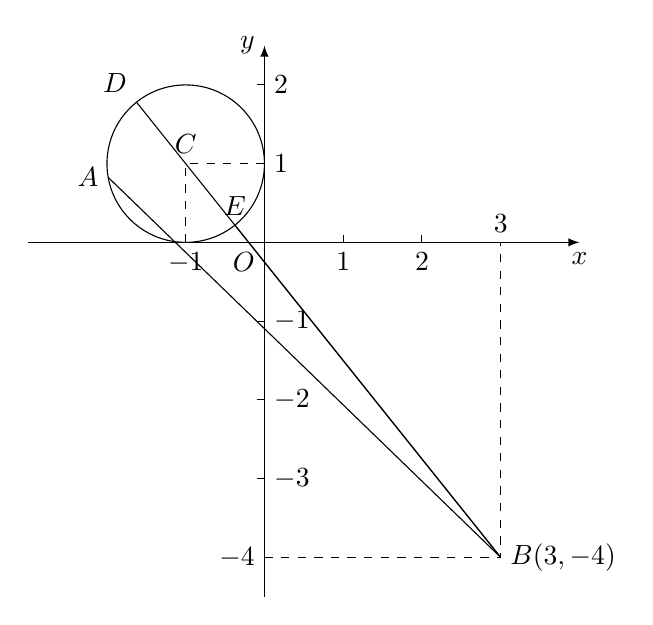
\begin{tikzpicture}[>=latex]
        \draw [->] (-3,0) -- (4,0) node [below] {$x$};
        \draw [->] (0,-4.5) -- (0,2.5) node [left] {$y$};
        \draw (0,0) node [below left] {$O$};
        \foreach \i in {-3,-2,-1,1,2} {\draw (-0.1,\i) -- (0,\i) node [right] {$\i$};};
        \draw (0.1,-4) -- (0,-4) node [left] {$-4$};
        \foreach \i in {-1,1,2} {\draw (\i,0.1) -- (\i,0) node [below] {$\i$};};
        \draw (3,0) node [above] {$3$};
        \draw [dashed] (-1,0) -- (-1,1) -- (0,1);
        \draw (-1,1) node [above] {$C$} coordinate (C) circle (1);
        \draw [dashed] (0,-4) -- (3,-4) node [right] {$B(3,-4)$} coordinate (B) -- (3,0);
        \draw (B) -- ($(B)!{1+1/sqrt(41)}!(C)$) node [above left] {$D$};
        \draw (B) -- ($(B)!{1-1/sqrt(41)}!(C)$) node [above] {$E$};
        \draw (C) ++ (190:1) node [left] {$A$} -- (B);
    \end{tikzpicture}
\end{center}
注意  设复数$z_0$, $z_1$, $z_2$在复平面内的对应点分别为$Z_0$, $Z_1$, $Z_2$, 则:
\textcircled{1} $|z-z_1|=|z-z_2|$表示线段$Z_1Z_2$的中垂线;
\textcircled{2} $|z-z_0|=R$($R>0$)表示以$Z_0$为圆心, $R$为半径的圆;
\textcircled{3} $|z-z_1|+|z-z_2|=2a$($2a>|Z_1Z_2|$)表示以$Z_1$, $Z_2$为焦点, $a$为半长轴的椭圆;
\textcircled{4} $||z-z_1|-|z-z_2||=2a$($0<2a<|Z_1Z_2|$)表示以$Z_1$, $Z_2$为焦点, $a$为半实轴长的双曲线.
\item 已知$|z_1|=|z_2|=1$, $z_1+z_2=\dfrac 12+\dfrac{\sqrt 3}2\mathrm{i}$, 求复数$z_1$, $z_2$.
解  如图,
\begin{center}
    \begin{tikzpicture}[>=latex,scale =2]
        \draw [->] (-1.5,0) -- (1.5,0) node [below] {$x$};
        \draw [->] (0,-1.5) -- (0,1.5) node [left] {$y$};
        \draw (0,0) node [below left] {$O$};
        \draw [->] (0,0) -- (1,0) node [below right] {$A$} coordinate (A);
        \draw [->] (0,0) -- (60:1) node [above] {$C$} coordinate (C);
        \draw [->] (0,0) -- (120:1) node [above] {$B$} coordinate (B);
        \draw (A) -- (C) -- (B);
        \draw (0,0) circle (1);
    \end{tikzpicture}
\end{center}
∵$z_1+z_2=\dfrac 12+\dfrac{\sqrt 3}2i$,
∴$z_1+z_2$对应于向量$\overrightarrow{OC}$, 其中$\angle COA=60^{\circ }$.
设$\overrightarrow{OA}$对应于复数$z_1$, $\overrightarrow{OB}$对应于复数$z_2$, 则四边形$AOBC$是菱形, 且$\triangle AOC$和$\triangle BOC$都是等边三角形, 于是$z_1=1$, $z_2=-\dfrac 12+\dfrac{\sqrt 3}3\mathrm{i}$或$z_1=-\dfrac 12+\dfrac{\sqrt 3}3\mathrm{i}$, $z_2=1$.
注意  复平面内, 若非零复数$z_1$, $z_2$分别对应于点$A$, $B$, $z_1+z_2$对应于点$C$, $O$为原点, 则:
\textcircled{1} $OACB$是平行四边形;
\textcircled{2} 若$|z_1|=|z_2|$, 则$OACB$是菱形;
\textcircled{3} 若$|z_1+z_2|=|z_1-z_2|$, 则$OACB$是矩形;
\textcircled{4} 若$|z_1|=|z_2|$且$|z_1+z_2|=|z_1-z_2|$, 则$OACB$是正方形.
\item 应用乘法公式解题.
应用下列两组乘法公式, 将会给计算带来便利:
(1)$(1+i)^2=2i$, $(1-i)^2=-2i$.
(2)记$\omega =-\dfrac 12\pm \dfrac{\sqrt 3}2i$, $\omega _1=-\dfrac 12+\dfrac{\sqrt 3}2i$, $\omega _2=-\dfrac 12-\dfrac{\sqrt 3}2i$,
则$\omega ^3=1$, $\omega ^2+\omega +1=0$, $\omega +\dfrac 1{\omega }=-1$, $\omega _1\omega _2=1$, $\omega _1^2=\omega _2$, $\omega _2^2=\omega _1$.
\item 求值:
(1)$(1+i)^{10}-(1-i)^{10}$.
(1)$\dfrac{{{(2+2i)}^5}}{{{(-1+\sqrt 3i)}^4}}$.
解  (1)原式$=[(1+i)^2]^5-[(1-i)^2]^5=(2i)^5-(-2i)^5=2^5i+2^5i=64i$.
(2)原式$=\dfrac{(2+2i){{(1+i)}^4}}{{{(-\dfrac 12+\dfrac{\sqrt 3}2i)}^4}}=\dfrac{(2+2i){{(2i)}^2}}{-\dfrac 12+\dfrac{\sqrt 3}2i}=\dfrac{-8(1+i)(-\dfrac 12-\dfrac{\sqrt 3}2i)}{(-\dfrac 12+\dfrac{\sqrt 3}2i)(-\dfrac 12-\dfrac{\sqrt 3}2i)}$
\blank{50}$=4(1+i)(1+\sqrt 3i)=4(1-\sqrt 3)+4(1+\sqrt 3)i$.
\item 应用复数模的运算法则解题.
容易证明, 复数模的运算有以下法则:
(1)$|z|=|\overline z|$, $|z_1\cdot z_2|=|z_1|\cdot|z_2|$, $|\dfrac{z_1}{z_2}|=|\dfrac{z_1}{z_2}|$($z_2\ne 0$), $|z^n|=|z|^n$.
(2)$|z|^2=z\cdot \overline z$.
\item 求复数$z=\dfrac{{{(3-4\mathrm{i})}^3}}{(\dfrac{\sqrt 3}2-\dfrac 12\mathrm{i})\cdot {{(\sqrt 3+\sqrt 2\mathrm{i})}^4}}$的模.
解  $|z|=\dfrac{{{|3-4i|}^3}}{{{|\dfrac{\sqrt 3}2-\dfrac 12i|}^2}\cdot {{|\sqrt 3+\sqrt 2i|}^4}}=\dfrac{5^3}{{{(\sqrt 5)}^4}}=5$.
\item 已知$|z|\le 1$, $|\omega|\le 1$, 求证: $|z+\omega|\le|1+\overline z\omega|$.
证明  ∵$|z+\omega|^2-|1+\overline z\omega|^2=(z+\omega)(\overline z+\overline \omega)-(1+\overline z\omega)(1+z\overline \omega)$
$=z\overline z+\omega \overline \omega -1-z\overline z\omega \overline \omega =|z|^2+|\omega|^2-1-|z|^2\cdot|\omega|^2=(|z|^2-1)(1-|\omega|^2)\le 0$.
∴$|z+\omega|^2\le|1+\overline z\omega|^2$, 于是$|z+\omega|\le|1+\overline z\omega|$.
\item 应用$z\in \mathbf{R}$的充要条件解题.
复数$z\in R$的充要条件是$z=\overline z$.
\item 若复数$z$满足$z+\dfrac 4z\in \mathbf{R}$, 且$|z-2|=2$, 求$z$.
解  ∵$z+\dfrac 4z\in \mathbf{R}$, ∴$z+\dfrac 4z=\overline z+\dfrac 4{\overline z}$, 整理得$z^2\overline z+4\overline z=z\overline{z^2}+4z$,
即$z|z|^2-|z|^2\cdot \overline z-4(z-\overline z)=0$, 即$(z-\overline z)(|z|^2-4)=0$.
(1)若$|z|=2$, 结合已知条件, $|z-2|=2$, 得$z=1\pm \sqrt 3i$.
(2)若$z-\overline z=0$, 结合$|z-2|=2$, 得$z=0$(舍去)和$z=4$.
综合(1)与(2), 得$z=1\pm \sqrt 3i$或$z=4$.
\item 应用不等式$||z_1|-|z_2||\le|z_1+z_2|\le|z_1|+|z_2|$解题.
\item 求函数$y=\sqrt {4a^2+x^2}+\sqrt {(x-a)^2+a^2}$($a>0$)的最值.
解  令$z_1=x+2ai$, $z_2=a-x+ai$,
则$y=|z_1|+|z_2|\ge|z_1+z_2|=|a+3ai|=\sqrt {10}a$.
∴当$\dfrac{a-x}x=\dfrac a{2a}$, 即$x=\dfrac{2a}3$时, 函数$y$有最小值$\sqrt {10}a$.
\item 若$|z+\dfrac 1z|=1$, 求$|z|$的取值范围.
解  由$||z|-|\dfrac 1z||\le|z+\dfrac 1z|$, 得$-1\le|z|-\dfrac 1{|z|}\le 1$,
即$\begin{cases}|z|^2+|z|-1\ge 0, \\|z|^2-|z|-1\le 0, \end{cases}$∴$\dfrac{\sqrt 5-1}2\le|z|\le \dfrac{\sqrt 5+1}2$.
注意  在应用不等式$||z_1|-|z_2||\le|z_1+z_2|\le|z_1|+|z_2|$求函数的最大值、最小值时, 需留意取``$=$''的条件.当$\overrightarrow{OZ_1}$与$\overrightarrow{OZ_2}$同向时, $|z_1+z_2|=|z_1|+|z_2|$; 当$\overrightarrow{OZ_1}$与$\overrightarrow{OZ_2}$异向时, $|z_1+z_2|=||z_1|-|z_2||$.
【训练题】
(一)复数的加法与减法
\item 两个共轭虚数的差一定是\bracket{20}.
\fourch{非零实数}{零}{纯虚数}{非纯虚数}
\item 复平面内, 已知复数$2-\mathrm{i}$和$3+4\mathrm{i}$分別对于点$M,N$, 则向量$\overrightarrow{MN}$对应的复数是\bracket{20}.
\fourch{$5+3i$}{$-1-5i$}{$1+5i$}{$1-5i$}
\item 若复数$z=3+a\mathrm{i}$满足条件$|z-2|<2$, 则实数$a$的取值范围是\bracket{20}.
\fourch{$(-2\sqrt 2,2\sqrt 2)$}{(-2, 2)}{(-1, 1)}{$(-\sqrt 3,\sqrt 3)$}
\item 若复数$z$满足$|z+3-4\mathrm{i}|=2$, 则$|z|$的最小值和最大值分别是\bracket{20}.
\fourch{1和9}{4和10}{5和11}{3和7}
\item (1)若$|z-25i|\le 15$, $z\in \mathbf{C}$, 则$|z|$最小时的$z=$\blank{50}, $|z|$最大时的$z=$\blank{50}.
(2)若复数$z$满足$|z|=3$, 则$|z-1+\sqrt 3\mathrm{i}|$的最小值是\blank{50}.
(3)若如数$z$满足$|z-3|=5$, 则$|z-(1+4i)|$的最大值是\blank{50}, 最小值是\blank{50}.
(4)若$|z-1-2i|=1$, 则$|z-3-i|$的取值范围是\blank{50}.
\item 复平面内, 已知点$A,B,C$分别对应于复数$z_1=1+\mathrm{i}$, $z_2=5+\mathrm{i}$, $z_3=3+3\mathrm{i}$, 以$AB,AC$为邻边作一平行四边形$ABDC$, 求点$D$对应的复数$z_4$及$AD$的长.
\item 若$f(\overline{z+i})=2z+\overline z+i$, 则$f(i)$等于\bracket{20}.
\fourch{1}{-1}{$i$}{$-i$}
\item 若复数$z$满足$|z+1|^2-|z+\mathrm{i}|^2=1$, 则$z$在复平面内的对应点所表示的图形是\bracket{20}.
\fourch{直线}{圆}{椭圆}{双曲线}
\item 若复数$z$满足$|z-1|+|z+1|=2$, 则$z$在复平面内的对应点所表示的图形是\bracket{20}.
\fourch{圆}{椭圆}{双曲线}{线段}
\item 若$z_1,z_2$都是虚数, 则``$z_1=\overline z_2$''的一个必要不充分条件是\bracket{20}.
\fourch{$|z_1-\overline z_2|=0$}{$\overline z_1=z_2$}{$z_1=z_2$}{$|z_1|=|z_2|$}
\item 复平面内, 曲线$|z-1+i|=1$关于直线$y=x$的对称曲线方程为\bracket{20}.
\fourch{$|z-1-i|=1$}{$|\overline z-1-i|=1$}{$|z+1+i|=1$}{$|\overline z+1+i|=1$}
\item 若$|z|=1$, 则$|z+i|+|z-6|$的最小值等于\bracket{20}.
\fourch{7}{$\sqrt {37}$}{6}{5}
\item (1)若复平面内的点$A,B$分别对应于复数$2+\mathrm{i}$和$1-\mathrm{i}$, 则线段$AB$的中垂线方程的复数形式是\blank{50}.
(2)设$z\in \mathbf{C}$, 则方程$|z+2|+|z-2|=6$对应的曲线的普通方程是\blank{50}.
(3)以$(\pm 3,0)$为两焦点, 且长半轴长为5的椭圆方程的复数形式是\blank{50}.
(4)已知复数$z$满足$|z-(1+i)|-|z-(1-i)|=2$, 则复平面内$z$的对应点的轨迹是\blank{50}.
(5)若$|z-3|+|z+3|=10$, 且$|z-5\mathrm{i}|-|z+5\mathrm{i}|=8$, 则复数$z=$\blank{50}.
(6)若$|z-2|=\sqrt {17}$, $|z-3|=4$, 则复数$z=$\blank{50}.
\item (1)设$|z_1|=3$, $|z_2|=5$, $|z_1+z_2|=6$, 求$|z_1-z_2|$.
(2)若$|z_1|=3$, $|z_1+z_2|=5$, $|z_1-z_2|=7$, 求$|z_2|$.
\item (1)已知两个复数集合$A=\{z||z-2|\le 2\}$, $B=\{z|z=\dfrac{z_1}2\mathrm{i}+b,z_1\in A,b\in R\}$.
\textcircled{1} 当$b=0$时, 求集合$B$所对应的区域;
\textcircled{2} 当$A\cap B=\varnothing$时, 求$b$的取值范围.
(2)若复数$z_1=1+2a\mathrm{i}$, $z_2=a+\mathrm{i}$($a\in R$), 集合$A=\{z||z-z_1|\le \sqrt 2\}$, $B=\{z||z-z_2|\le 2\sqrt 2\}$满足$A\cap B=\varnothing$, 求$a$的取值范围.
\item (1)已知复数$z_1,z_2$满足$|z_1|=1$, $|z_2|=1$, 且$z_1+z_2=\dfrac 12+\dfrac{\sqrt 3}2i$, 求$z_1,z_2$.
(2)复平面内三点$A,B,C$依次对应于复数$1+z$, $1+2z$, $1+3z$, 其中$|z|=2$, $O$为原点, 若$S_{\triangle AOB}+S_{\triangle BOC}=2$, 求复数$z$.
(二)复数的乘法与除法
\item 若复数$z=(1+\mathrm{i})^2$, 则$z\cdot \overline z$的值为\bracket{20}.
\fourch{$-4i$}{$4i$}{4}{8}
\item 计算$(\dfrac{\sqrt 2i}{1+i})^{100}$的结果是\bracket{20}.
\fourch{$i$}{$-i$}{1}{-1}
\item 当$n$取遍正整数时, $i^n+i^{-n}$表示不同值的个数是\bracket{20}.
\fourch{1}{2}{3}{4}
\item 使$(\dfrac{1+i}{1-i})^n$为实数的最小自然数$n$是\bracket{20}.
\fourch{2}{4}{6}{8}
\item ``$z_1$和$z_2$为共轭复数''是``$z_1+z_2\in R$且$z_1\cdot z_2\in R$''的\bracket{20}.
\fourch{充分不必要条件}{必要不充分条件}{充要条件}{既不充分也不必要条件}
\item 若$(z-1)^2=|z-1|^2$, 则$z$一定是\bracket{20}.
\fourch{纯虚数}{实数}{虚数}{零}
\item 设$z=1+ki$($k\in \mathbf{R}$), 则$z^2$对应点的轨迹是\bracket{20}.
\fourch{圆}{椭圆}{抛物线}{双曲线}
\item 若都是$z$, $z_1$, $z_2$复数, 判断下列命题的真假:
(1)$|z|^2=z^2$.\bracket{20}.					(2)$|z|^2\ne z^2$.\bracket{20}.
(3)$|z^2|=|z|^2$.\bracket{20}.					(4)$|z|\le 1\Leftrightarrow -1\le z\le 1$.\bracket{20}.
(5)$\sqrt {|z|^2}=|z|$.\bracket{20}.					(6)若$|z_1|=|z_2|$, 则$z_1=\pm z_2$.\bracket{20}.
(7)$z+\overline z$是实数.\bracket{20}.				(8)$z-\overline z$是纯虚数.\bracket{20}.
(9)$z^2\ge 0$.\bracket{20}.						(l0)若$|z|=1$, 则$\overline z=\dfrac 1z$.\bracket{20}.
(11)$z=\overline z\Leftrightarrow z\in \mathbf{R}$.\bracket{20}.			(12)若$z_1^2+z_2^2=0$, 则$z_1=z_2=0$.\bracket{20}.
\item (1)$(i-\dfrac 1i)^6$的虚部是\blank{50}.
(2)计算$(1+i)^{20}-(1-i)^{20}=$\blank{50}.
(3)计算$\dfrac{{{(1+i)}^5}}{1-i}+\dfrac{{{(1-i)}^5}}{1+i}=$\blank{50}.
(4)若$z=1+i$, 则$\dfrac 5{1+z^2}=$\blank{50}.
(5)计算$\dfrac{-2\sqrt 3+i}{1+2\sqrt 3i}+(\dfrac{\sqrt 2}{1+i})^{3996}=$\blank{50}.
(6)若$a\in \mathbf{R}$, 且$\dfrac{a+2i}{3+i}\in \mathbf{R}$, 则$\dfrac{a+2i}{3+i}=$\blank{50}.
\item (1)已知$\omega =-\dfrac 12+\dfrac{\sqrt 3}2i$, 则: \textcircled{1} $\omega ^2+\dfrac 1{\omega ^2}=$\blank{50}; \textcircled{2} $\omega ^3+\dfrac 1{\omega ^3}=$\blank{50}.
\textcircled{3} $\omega ^{14}+\dfrac 1{\omega ^{14}}=$\blank{50}; \textcircled{4} $1+\omega +\omega ^2+\omega ^3+\cdots +\omega ^{10}=$\blank{50}.
(2)若$f(x)=2x^4-11x^3-7x^2-9x+4$, 则$f(-\dfrac 12+\dfrac{\sqrt 3}2i)=$\blank{50}.
\item 计算下列各题:
(1)$(i-\dfrac 1i)^{10}=$\blank{50}.
(2)$\dfrac{{{(1+i)}^3}-{{(1-i)}^3}}{{{(1+i)}^2}-{{(1-i)}^2}}=$\blank{50}.
(3)$i\cdot i^2\cdot i^3\cdot \cdots \cdot i^{1997}=$\blank{50}.
(4)$i+i^2+i^3+\cdots +i^{1997}=$\blank{50}.
(5)$(\dfrac{1+i}{\sqrt 2})^{1997}+(\dfrac{1-i}{\sqrt 2})^{1997}=$\blank{50}.
\item 已知$i^{3m}=i^n$($m,n\in \mathbf{Z}$), 则$i^{m+n}$的值为\bracket{20}.
\fourch{1}{$i$}{$-i$}{-1}
\item 若$x+\dfrac 1x=-1$, 则$x^{17}+x^{-17}$的值等于\bracket{20}.
\fourch{0}{-1}{1}{2}
\item (1)计算: $1+2i+3i^2+4i^3+\cdots +10i^9$.
(2)计算:  $i+2i^2+3i^3+\cdots +359i^{359}$.
(3)求首项为$i$, 公比为$1+\dfrac 1i$的等比数列的第七项.
\item (1)计算:
\textcircled{1} $(\dfrac{-1+i}{1+\sqrt 3i})^3$; 							\textcircled{2} $\dfrac{{{(\sqrt 3+i)}^5}}{-1+\sqrt 3i}$.
(2)求下列复数的模:
\textcircled{1} $(3+4i)(-\dfrac 12+\dfrac{\sqrt 3}2i)$; 					\textcircled{2} $\dfrac{5-12i}{-8+15i}$;
\textcircled{3} $\dfrac{{{(1+i)}^3}}{{{(1-i)}^2}(9+40i)}$; 						\textcircled{4} $\dfrac{1-{t^2}}{1+{t^2}}+\dfrac{2t}{1+{t^2}}i$($t\in \mathbf{R}$);
\textcircled{5} $\dfrac{{{(1-i)}^{10}}{{(3-4i)}^4}}{{{(-\sqrt 3+i)}^8}}$; 						⑥$\dfrac{(\sqrt 6+i){{(1+i)}^2}}{(-1+\sqrt 6i)(-\dfrac 13+\dfrac{2\sqrt 2}3i)(\sqrt 3i)}$.
\item 已知$z=1+i$, 且$\dfrac{{z^2}+az+b}{{z^2}-z+1}=1-i$, 求实数$a,b$的值.
\item 已知$a>0$, 且$a\ne 1$, 若$(\log _ax+i)z=1+i\log _ax$, 问: $x$为何值时, $z$为:
(1)实数.		(2)虚数.			(3)纯虚数.			(4)模等于1的复数.
\item (1)已知$z=|\dfrac{\sqrt 2i{{(3+i)}^2}}{{{(\sqrt 3+\sqrt 7i)}^2}}|+2i$, 求$|z|$.
(2)已知复数$z=\dfrac{{{(1+\mathrm{i})}^3}{{(a-1)}^2}}{\sqrt 2{{(a-3\mathrm{i})}^2}}$满足$|z|=\dfrac 23$, 求实数$a$的值.
(3)已知复数$z$满足$|z|=5$, 且$(3+4i)z$是纯虚数, 求$z$.
(4)已知$z=\dfrac{\sqrt 3\sin \theta +i\cos \theta }{\sin \theta -i\sqrt 3\cos \theta }$, 求$z$的最大值.
(5)已知复数$z$满足$|z+\dfrac 1z|=1$, 求$|z|$的取值范围.
\item (1)已知复数$z$满足$z+\dfrac 4z\in \mathbf{R}$, $|z-2|=2$, 求$z$.
(2)已知复数$z$满足$|z-4|=|z-4\mathrm{i}|$, $z+\dfrac{14-z}{z-1}\in R$, 求$z$.
(3)已知$|\dfrac{z-12}{z-8i}|=\dfrac 53$, $|\dfrac{z-4}{z-8}|=1$, 求复数$z$.
\item 根据条件, 求复数$z$在复平面内的对应点轨迹的普通方程:
(1)$z^2+\dfrac 9{z^2}\in \mathbf{R}$.	(2)$\dfrac z{z-1}$为纯虚数.		(3)$z\cdot \overline z+az+\overline z=0$($a\in \mathbf{R}$).
\item 已知非零夏数$z_1,z_2$满足$|z_1+z_2|=|z_1-z_2|$, 求证: $(\dfrac{z_1}{z_2})^2$一定是负数.
\item (1)已知$P,Q$两点分别对应于复数$z_1$和$2z_1+3-4\mathrm{i}$, 若点$P$在曲线$|z|=2$上移动, 求点$Q$的轨迹.
(2)已知复数$z$满足$|z|=2$, 求复数$\omega =\dfrac{z+1}z$在复平面内的对应点的轨迹.
(3)复平面内两动点$P_1,P_2$所对应的复数$z_1,z_2$满足$z_1=z_2\mathrm{i}+3$, 又点$P_2$沿着曲线$|z-5|-|z+5|=6$运动, 试求点$P_1$的轨迹方程, 并指出它表示何种曲线.
(4)复平面内, 线段$AB$上的点$P$对应的复数为$z$, 其中$A,B$点分别对应于复数$z_A=1$, $z_B=i$, 求$z^2$的对应点轨迹的普通方程, 并画出图形.
(5)已知点$Q(u,v)$在$O(0,0)$, $A(1,0)$, $B(1,1)$为顶点的$\triangle OAB$的边界上移动, 求$z=(u+2vi)^2+2+3i$所对应的点$P$的轨迹, 并画出草图.
\item 求证:
(1)复数$z$可以表示为$\dfrac{1+t\mathrm{i}}{1-t\mathrm{i}}$($t\in R$)的充要条件是$|z|=1$且$z\ne -1$.
(2)$\dfrac{z-1}{z+1}$为纯虚数的充要条件是$|z|=1$且$z\ne \pm 1$.
\item 利用$||z_1|-|z_2||\le|z_1+z_2|\le|z_2|+|z_2|$解下列各题:
(1)求函数$y=\sqrt {x^2+4}+\sqrt {x^2-8x+17}$的最小值及相应的$x$.
(2)求函数$y=\sqrt {x^2+9}-\sqrt {x^2-2x+5}$的最大值及相应的$x$.
(3)求证: $\sqrt {x^2+y^2}+\sqrt {(x-2)^2+y^2}+\sqrt {x^2+(y-2)^2}+\sqrt {(x-2)^2+(y-2)^2}\ge 4\sqrt 2$.
\item 利用$|z|^2=z\cdot \overline z$解下列各题: .
(1)若$|z|=1$, 求证$|\dfrac{a-z}{1-a\overline z}|=1$.
(2)若$|1-z_1z_2|=|z_1-\overline z_2|$, 求证: $|z_1|$, $|z_2|$中至少有一个为1.
(3)若$|z_1|\le 1$, $|z_2|\le 1$, 求证: $|\dfrac{{z_1}-{z_2}}{1-{{\overline z}_1}{z_2}}|\le 1$.
(4)若复数$z_{\mathrm{i}}$满足$|z_{\mathrm{i}}|=1$($\mathrm{i}=1,2,3$), 求$|\dfrac{{z_1}{z_2}+{z_2}{z_3}+{z_3}{z_1}}{{z_1}+{z_2}+{z_3}}|$的值.
(5)已知复数$A=z_1\overline z_2+z_2\overline z_1$, $B=z_1\overline z_1+z_2\overline z_2$, 其中$z_1,z_2$是非零复数, 问: $A,B$可不可以比较大小? 并证明之.
\item (1)已知$|z|=1$, $|z_2|=\sqrt 2$, 求证: $|\dfrac{2{z_1}+(1+3i)z_2^2}{3+4i}|\le \dfrac{12}5$.
(2)已知$z=\dfrac{\sin \alpha +i\sqrt 2\cos \alpha }{\sqrt 2\sin \alpha -i\cos \alpha }$, 求证: $\dfrac{\sqrt 2}2\le|z|\le \sqrt 2$.
(3)复平面内三点$A,B,C$分别对应于复数$z_1,z_2,z_3$, 若$\dfrac{{z_2}-{z_1}}{{z_3}-{z_1}}=1+\dfrac 43\mathrm{i}$, 试求$\triangle ABC$的三边之比.
\item 已知$|z|=1$, 求下列各式的最大值和最小值:
(1)$|z^2-z+1|$.		(2)$|z^2-z+2|$.		(3)$|z^3-3z-2|$.
三、复数的三角形式
【典型题型和解题技巧】
\item 复数的三角形式.
(1)``伪三角形式''化为三角形式.
复数的三角形式是$r(\cos \theta +\mathrm{i}\sin \theta)$($r\ge 0$), 读者需能熟练地将下列各``伪三角形式, , 化为三角形式($r>0$):
$r(\cos \theta -i\sin \theta)=[\cos (-\theta)+i\sin (-\theta)]$, $r(-\cos \theta +i\sin \theta)=[\cos (\pi -\theta)+i\sin (\pi -\theta)]$, $-r(\cos \theta +i\sin \theta)=r[\cos (\pi +\theta)+i\sin (\pi +\theta)]$,
$r(\sin \theta +i\cos \theta)=r[\cos (\dfrac{\pi }2-\theta)+i\sin (\dfrac{\pi }2-\theta)]$.
\item 将下列复数化为三角形式:
(1)$2(\cos \dfrac{\pi }5-i\sin \dfrac{\pi }5)$.					(2)$2(-\cos \dfrac{\pi }5+i\sin \dfrac{\pi }5)$.
(3)$-2(\cos \dfrac{\pi }5+i\sin \dfrac{\pi }5)$.					(4)$2(\sin \dfrac{\pi }5+i\cos \dfrac{\pi }5)$.
解  (1)$2(\cos \dfrac{\pi }5-i\sin \dfrac{\pi }5)=2[\cos (-\dfrac{\pi }5)+i\sin (-\dfrac{\pi }5)]$.
(2)$2(-\cos \dfrac{\pi }5+i\sin \dfrac{\pi }5)=2(\cos \dfrac{4\pi }5+i\sin \dfrac{4\pi }5)$.
(3)$-2(\cos \dfrac{\pi }5+i\sin \dfrac{\pi }5)=2(\cos \dfrac{6\pi }5+i\sin \dfrac{6\pi }5)$.
(4)$2(\sin \dfrac{\pi }5+i\cos \dfrac{\pi }5)=2(\cos \dfrac{3\pi }{10}+i\sin \dfrac{3\pi }{10})$.
(2)代数形式化为三角形式.
将复数的代数形式$z=a+b\mathrm{i}$($a,b\in R$)化为三角形式$z=r(\cos \theta +\mathrm{i}\sin \theta)$($r>0$), 可按如下步骤进行:
\textcircled{1} 画图, 并标出$r$和$\theta$;
\textcircled{2} 求$\theta$和$r$, 其中$r=\sqrt {a^2+b^2}$, $\cos \theta =\dfrac ar$, $\sin \theta =\dfrac br$;
\textcircled{3} 写出$z$的三角形式.
\item 将下列复数化成三角形式:
(1)$z=-\sqrt 3+i$.					(2)$5-12i$.
解  (1)如下图,
∵$r=2$, $\cos \theta =-\dfrac{\sqrt 3}2$, $\theta =\dfrac{5\pi }6$, ∴$-\sqrt 3+i=2(\cos \dfrac{5\pi }6+i\sin \dfrac{5\pi }6)$.
\begin{center}
    \begin{tikzpicture}[>=latex]
        \draw [->] (-2,0) -- (2,0) node [below] {$x$} coordinate (X);
        \draw [->] (0,-2) -- (0,2) node [left] {$y$};
        \draw (0,0) coordinate (O) node [below left] {$O$};
        \draw (150:2) node [above] {$(-\sqrt{3},1)$} coordinate (T);
        \draw [->] (O) -- (T);
        \draw ($(T)!0.5!(O)$) node [above] {$r$};
        \draw [dashed] (0,1) node [right] {$1$}-- (T) -- ({-sqrt(3)},0) node [below] {$-\sqrt{3}$};
        \pic (O) [draw,->] {angle = X--O--T};
        \draw (37:0.4) node [above right] {$\theta$};
    \end{tikzpicture}
    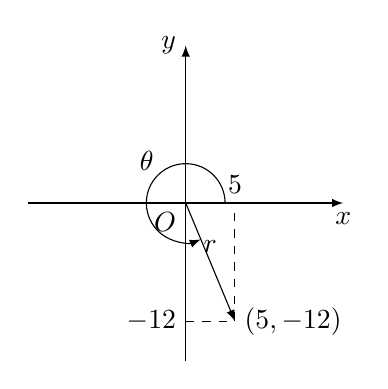
\begin{tikzpicture}[>=latex]
        \draw [->] (-2,0) -- (2,0) node [below] {$x$} coordinate (X);
        \draw [->] (0,-2) -- (0,2) node [left] {$y$};
        \draw (0,0) coordinate (O) node [below left] {$O$};
        \draw ({5/8},{-12/8}) node [right] {$(5,-12)$} coordinate (T);
        \draw [->] (O) -- (T);
        \draw ($(T)!0.5!(O)$) node [above] {$r$};
        \draw [dashed] (0,{-12/8}) node [left] {$-12$} -- (T) -- ({5/8},0) node [above] {$5$};
        \pic (O) [draw,->] {angle = X--O--T};
        \draw (135:0.4) node [above left] {$\theta$};
    \end{tikzpicture}
\end{center}
(2)如上图,
∵$r=13$, $\cos \theta =\dfrac 5{13}$, $\theta =2\pi-\arccos \dfrac 5{13}$,
∴$5-12i=13[\cos (-\arccos \dfrac 5{13})+i\sin (-\arccos \dfrac 5{13})]$.
\blank{50}(1)\blank{50}(2)
(图4)
(3)复数的辐角、辐角主值$\arg z$.
需要时时记住的是复数$z$的辐角主值的取值范围是$[0,2\pi)$, $\arg z\in [0,2\pi)$.
\item 若复数$z=\dfrac 12+\mathrm{i}\sin \alpha$($\alpha \in R$), 且$|z|\le 1$, 求$\arg z$和$\alpha$的取值范围.
解  ∵$|z|\le 1$, ∴$\dfrac 14+\sin ^2\alpha \le 1$, ∴$-\dfrac{\sqrt 3}2\le \sin \alpha \le \dfrac{\sqrt 3}2$
如图, $z$的对应点$P$应在线段$AB$上运动, 当点$P$在$MA$上时, $\arg z\in [0,\dfrac{\pi }3]$, 当点$P$在$BM$上时, $\arg z\in [\dfrac{5\pi }3,2\pi)$.
\begin{center}
    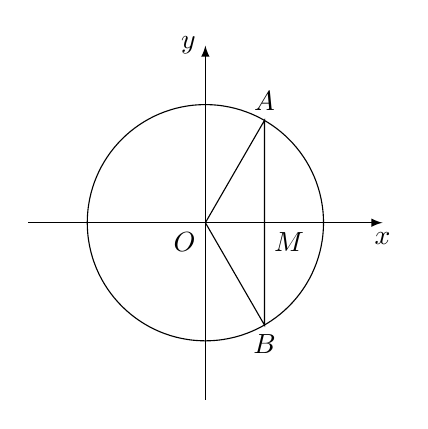
\begin{tikzpicture}[>=latex,scale = 1.5]
        \draw [->] (-1.5,0) -- (1.5,0) node [below] {$x$};
        \draw [->] (0,-1.5) -- (0,1.5) node [left] {$y$};
        \draw (0,0) node [below left] {$O$};
        \draw (0,0) circle (1);
        \draw (0.5,{sqrt(3)/2}) node [above] {$A$} -- (0.5,{-sqrt(3)/2}) node [below] {$B$} -- (0,0) -- cycle;
        \draw (0.5,0) node [below right] {$M$};
    \end{tikzpicture}
\end{center}
∴$\arg z\in [0,\dfrac{\pi }3]\cup [\dfrac{5\pi }3,2\pi)$.
∴$a\in [k\pi -\dfrac{\pi }3,k\pi +\dfrac{\pi }3]$($k\in \mathbf{Z}$).
\item 已知$z+\dfrac 1z=\cos x$($x\in \mathbf{R}$), 且$|z|\le 1$, 求$\arg z$的取值范围.
解  先设$|z|<1$, 则如图所示, 此时$z+\dfrac 1z$所对应的向量不在$x$轴上,
\begin{center}
    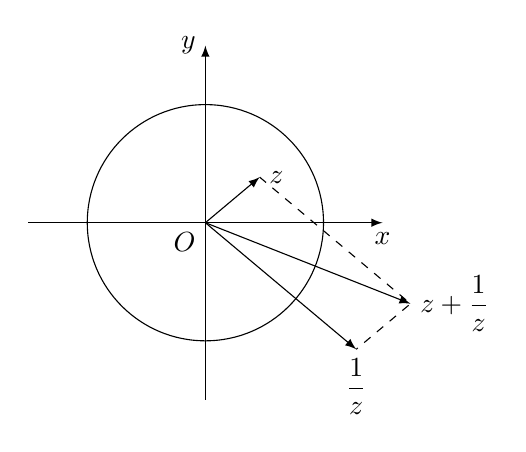
\begin{tikzpicture}[>=latex,scale=1.5]
        \draw [->] (-1.5,0) -- (1.5,0) node [below] {$x$};
        \draw [->] (0,-1.5) -- (0,1.5) node [left] {$y$};
        \draw (0,0) node [below left] {$O$};
        \draw (0,0) circle (1);
        \draw (40:0.6) coordinate (A);
        \draw (-40:{1/0.6}) coordinate (B) ++ (40:0.6) coordinate (C);
        \draw [->] (0,0) -- (A) node [right] {$z$};
        \draw [->] (0,0) -- (B) node [below] {$\dfrac 1 z$};
        \draw [->] (0,0) -- (C) node [right] {$z+\dfrac 1z$};
        \draw [dashed] (A) -- (C) -- (B); 
    \end{tikzpicture}
\end{center}
∴$z+\dfrac 1z\ne \cos x$,
故$|z|<1$不可能, 于是$|z|=1$.
令$z=\cos \theta +i\sin \theta$($0\le \theta <2\pi$),
则由$z+\dfrac 1z=z+\overline z=2\cos \theta =\cos x$,
得$\cos \theta =\dfrac 12\cos x\in [-\dfrac 12,\dfrac 12]$.
∴$\theta \in [\dfrac{\pi }3,\dfrac{2\pi }3]\cup [\dfrac{4\pi }3,\dfrac{5\pi }3]$, 即$\arg z\in [\dfrac{\pi }3,\dfrac{2\pi }3]\cup [\dfrac{4\pi }3,\dfrac{5\pi }3]$.
\item 应用复数的三角形式解题.
若题目给出了$|z|=r$($r>0$)的条件, 一般来说, 复数的三角形式当是解题的最佳选择了, 即可令$z=r(\cos \theta +i\sin \theta)$.特别地, 若$|z|=1$, 则可令$z=\cos \theta +i\sin \theta$.
\item 已知非零复数$z$满足$|z-\mathrm{i}|=1$, 且$\arg z=\theta$, 求:
(1)$\theta$的取值范围.	(2)复数$z$的模.	(3)复数$z^2-zi$的辐角.
解  (1)∵$|z-i|=1$, ∴$z$的对应点$P$在以(0, 1)为圆心, 半径为1的圆上(如下图左), $\theta$的取值范围是$0<\theta <\pi$.
(2)如下图中, 在Rt$\triangle AOP$中,
∵$|OP|=2\sin \theta$, 故$|z|=2\sin \theta$.
(3)由$|z-i|=1$, 故可令$z-i=\cos \varphi +i\sin \varphi$($\varphi \in \mathbf{R}$),
于是$z^2-zi=z(z-i)=2\sin \theta (\cos \theta +i\sin \theta)\cdot (\cos \varphi +i\sin \varphi)=2\sin \theta [\cos (\theta +\varphi)+i2\sin (\theta +\varphi)]$.又$\cos \varphi +i\sin \varphi =z-i=2\sin \theta (\cos \theta +i\sin \theta)-i=2\sin \theta \cos \theta +i(2\sin ^2\theta -1)$
$=\sin 2\theta -i\cos 2\theta =\cos (2\theta -\dfrac{\pi }2)+i\sin (2\theta -\dfrac{\pi }2)$,
∴$\varphi =2k\pi +2\theta -\dfrac{\pi }2$($k\in \mathbf{Z}$), $\theta +\varphi =2k\pi +3\theta -\dfrac{\pi }2$($k\in \mathbf{Z}$).
即$\arg (z^2-zi)=2k\pi +3\theta -\dfrac{\pi }2$($k\in \mathbf{Z}$).
\begin{center}
    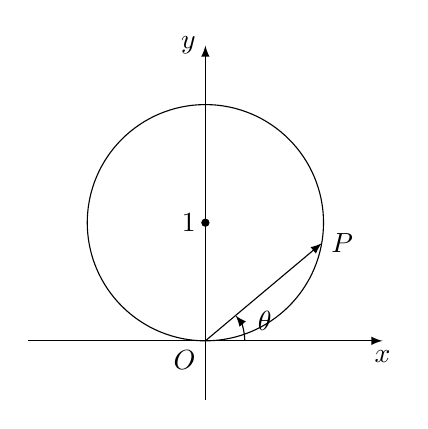
\begin{tikzpicture}[>=latex,scale = 1.5]
        \draw [->] (-1.5,0) -- (1.5,0) coordinate (X) node [below] {$x$};
        \draw [->] (0,-0.5) -- (0,2.5) node [left] {$y$};
        \draw (0,0) node [below left] {$O$};
        \draw (0,1) circle (1);
        \filldraw (0,1) circle (0.03) node [left] {$1$};
        \draw (0,1) ++ (-10:1) node [right] {$P$} coordinate (P);
        \draw [->] (0,0) coordinate (O) -- (P);
        \pic [draw, ->] {angle = X--O--P};
        \draw (25:0.4) node [right] {$\theta$};
    \end{tikzpicture}
    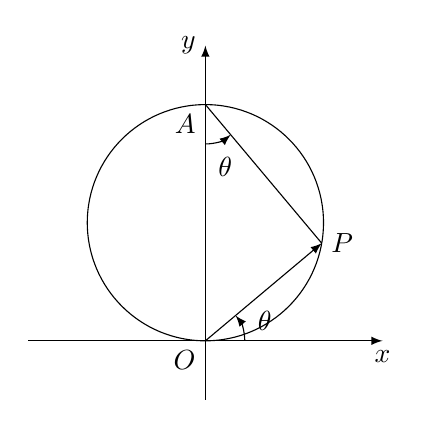
\begin{tikzpicture}[>=latex,scale = 1.5]
        \draw [->] (-1.5,0) -- (1.5,0) coordinate (X) node [below] {$x$};
        \draw [->] (0,-0.5) -- (0,2.5) node [left] {$y$};
        \draw (0,0) node [below left] {$O$};
        \draw (0,1) circle (1);
        \draw (0,2) node [below left] {$A$} coordinate (A);
        \draw (0,1) ++ (-10:1) node [right] {$P$} coordinate (P);
        \draw [->] (0,0) coordinate (O) -- (P);
        \draw (A) -- (P);
        \pic [draw, ->] {angle = X--O--P};
        \pic [draw, ->] {angle = O--A--P};
        \draw (25:0.4) node [right] {$\theta$};
        \draw (A) ++ (-65:0.4) node [below] {$\theta$};
    \end{tikzpicture}
    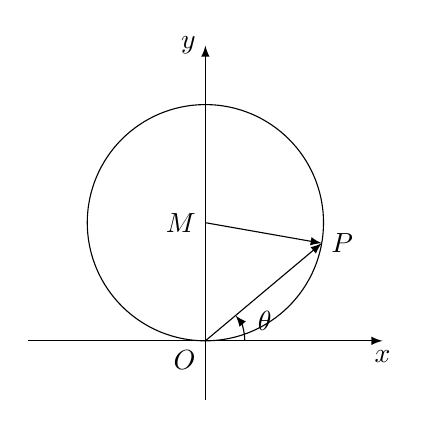
\begin{tikzpicture}[>=latex,scale = 1.5]
        \draw [->] (-1.5,0) -- (1.5,0) coordinate (X) node [below] {$x$};
        \draw [->] (0,-0.5) -- (0,2.5) node [left] {$y$};
        \draw (0,0) node [below left] {$O$};
        \draw (0,1) circle (1);
        \filldraw (0,1) node [left] {$M$} coordinate (M);
        \draw (0,1) ++ (-10:1) node [right] {$P$} coordinate (P);
        \draw [->] (0,0) coordinate (O) -- (P);
        \draw [->] (M) -- (P);
        \pic [draw, ->] {angle = X--O--P};
        \draw (25:0.4) node [right] {$\theta$};
    \end{tikzpicture}
\end{center}
第(3)题有另一种解法: 如上图右, $z-i$和向量$\overrightarrow{MP}$对应, 而$\angle OMP=2\theta$, 则$z-i$的一个辐角为$2\theta -\dfrac{\pi }2$, 由$z^2-zi=z(z-i)$知, $z^2-zi$的辐角等于$z$的辐角和$z-i$的辅角之和, 即$2k\pi +3\theta -\dfrac{\pi }2$($k\in \mathbf{Z}$).
注意  需要掌握的是对于已知$|z|=r$($r>0$)的有关问题, 可以从以下四个方面去思考;
(1)令$z=r(\cos \theta +i\sin \theta)$.
(2)令$z=a+bi$($a,b\in \mathbf{R}$), 且$a^2+b^2=r^2$.
(3)由$|z|^2=r^2$, 得$z\overline z=r^2$, $z=\dfrac{r^2}{\overline z}$, $\overline z=\dfrac{r^2}z$.
(4)$z$在复平面内的对应点在以原点为圆心, $r$为半径的圆上.有时候, 并不一定以三角形式为最佳.
\item 运用复数乘法、除法的几何意义解题.
若$u=z\cdot r(\cos \theta +i\sin \theta)$, 则只需将$\overrightarrow{OP}$($P$为$z$在复平面内的对应点)绕原点逆转$\theta$角, 并将$|\overrightarrow{OP}|$扩大到原来的$r$倍, 即得复数$u$的对应向量$\overrightarrow{OU}$.
若$u=\dfrac z{r(\cos \theta +i\sin \theta)}$, 则只需将$\overrightarrow{OP}$前绕原点顺转$\theta$角, 并将$\overrightarrow{OP}$缩小到原来的$r$倍, 即得$u$的对应向量$\overrightarrow{OU}$.
\item 已知等边$\triangle ABC$的两个顶点坐标是$A$(2, 1), $B$(3, 2), 求顶点$C$的对应坐标.
解  记$A,B,C$的对应复数为$z_A=2+\mathrm{i}$, $z_B=3+2\mathrm{i}$, $z_C$.
由$z_C=z_A+(z_B-z_A)[\cos 60^{\circ }\pm i\sin 60^{\circ }]$,
得$z_C=(2+i)+(1+i)(\dfrac 12\pm \dfrac{\sqrt 3}2i)=\dfrac{5\mp \sqrt 3}2+\dfrac{3\pm \sqrt 3}2i$,
即点$C$坐标是$(\dfrac{5-\sqrt 3}2+\dfrac{3+\sqrt 3}2)$或$(\dfrac{5+\sqrt 3}2+\dfrac{3-\sqrt 3}2)$.
\item 复平面内, 两点$A,B$分別对应于复数$\alpha ,\beta$, 且$\beta +(1+\mathrm{i})\alpha =0$, $|\alpha -2+\mathrm{i}|=1$, 求$\triangle AOB$面积的最大值和最小值.
解  ∵$|\alpha -(2-i)|=1$,
∴$A$是以$C(2,-1)$为圆心, 1为半径的圆上的动点.
而$\beta =(-1-i)\alpha =\sqrt 2(\cos \dfrac{5\pi }4+i\sin \dfrac{5\pi }4)\alpha$,
故线段$OB$的长是$OA$长的$\sqrt 2$倍, 且由$OA$绕原点按逆时针方向旋转$\dfrac{5\pi }4$而得(如图).
\begin{center}
    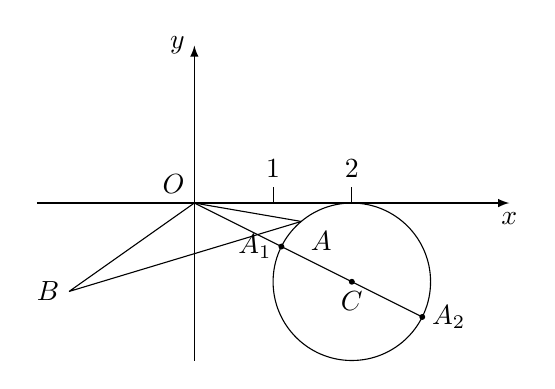
\begin{tikzpicture}[>=latex]
        \draw [->] (-2,0) -- (4,0) node [below] {$x$};
        \draw [->] (0,-2) -- (0,2) node [left] {$y$};
        \draw (0,0) coordinate (O) node [above left] {$O$};
        \draw (1,0) -- (1,0.2) node [above] {$1$};
        \draw (2,0) -- (2,0.2) node [above] {$2$};
        \draw (2,-1) circle (1);
        \filldraw (2,-1) circle (0.03) node [below] {$C$} coordinate (C);
        \draw (C) ++ (130:1) node [below right] {$A$} coordinate (A);
        \draw (O) -- (A);
        \draw ($(O)!{sqrt(2)}!-135:(A)$) coordinate (B) node [left] {$B$};
        \draw (A) -- (B) (O) -- (B);
        \draw ($(O)!{1-1/sqrt(5)}!(C)$) node [left] {$A_1$} coordinate (A1);
        \draw ($(O)!{1+1/sqrt(5)}!(C)$) node [right] {$A_2$} coordinate (A2);
        \draw (O) -- (A2);
        \filldraw (A1) circle (0.03) (A2) circle (0.03);
    \end{tikzpicture}
\end{center}
故$S_{\triangle AOB}=\dfrac 12|OA|\cdot|OB|\cdot \sin \dfrac{3\pi }4=\dfrac 12\sqrt 2\cdot|OA|^2\cdot \dfrac{\sqrt 2}2=\dfrac 12|OA|^2$.
连接$OC$并延长, 与圆交于点$A_1$, $A_2$, 则$|OA_1|=\sqrt 5-1$, $|OA_2|=\sqrt 5+1$, 因此$\triangle AOB$面积的最大值和最小值分别为$\dfrac 12(\sqrt 5+1)^2$和$\dfrac 12(\sqrt 5-1)^2$, 即$3+\sqrt 5$和$3-\sqrt 5$.
\item 已知定点$A(-2,0)$和圆$x^2+y^2=1$的动点$B$, 点$A,B,C$按逆时针方向排列, 且$|AB|:|BC|:|CA|=3:4:5$(如图12), 求点$C$的轨迹方程.
解  设点$C,B$分别对应复数$z,z_0$,
则$z=z_0+(-2-z_0)(-\dfrac 43i)=z_0+\dfrac 43iz_0+\dfrac 83i$,
于是$(1+\dfrac 43i)z_0=z-\dfrac 83i$, 两边取模得$|1+\dfrac 43i|\cdot|z_0|=|z-\dfrac 83i|$.
又∵$|z_0|=1$, ∴$|z-\dfrac 83i|=\dfrac 53$,
即点$C$的轨迹是以$(0,\dfrac 83)$为圆心, $\dfrac 53$为半径的圆.
\begin{center}
    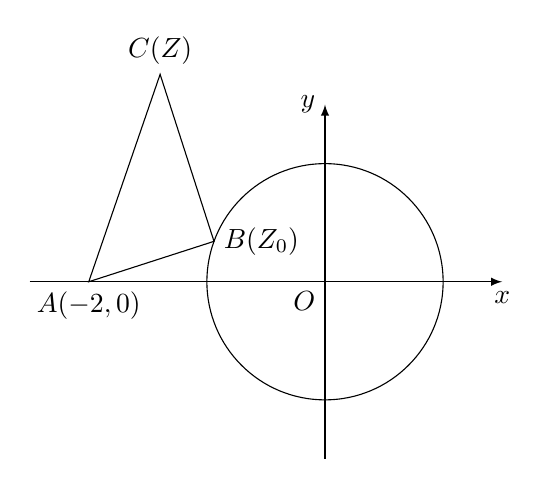
\begin{tikzpicture}[>=latex,scale = 1.5]
        \draw [->] (-2.5,0) -- (1.5,0) node [below] {$x$};
        \draw [->] (0,-1.5) -- (0,1.5) node [left] {$y$};
        \draw (0,0) node [below left] {$O$};
        \draw (0,0) circle (1);
        \draw (-2,0) node [below] {$A(-2,0)$} coordinate (A);
        \draw (160:1) node [right] {$B(Z_0)$} coordinate (B);
        \draw ($(B)!{4/3}!-90:(A)$) node [above] {$C(Z)$} coordinate (C);
        \draw (A) -- (B) -- (C) -- cycle; 
    \end{tikzpicture}
\end{center}
注意  (1)用复数知识求点的轨迹, 主要用于求从动点的轨迹问题, 常用``转移法''.
(2)本例解法中, 设主动点对应于复数$z_0$, 从动点对应于复数$z$, 有时, 则需设主动点对应于复数$x_0+y_0i$, 从动点对应于复数$x+yi$($x_0,y_0,x,y\in \mathbf{R}$).
\item 复数在三角中的应用.
\item 求值: $arc\cot \dfrac 13+\arcsin \dfrac 1{\sqrt {26}}+\arccos \dfrac 7{\sqrt {50}}+arc\cot 8$.
解  ∵$\arcsin \dfrac 1{\sqrt {26}}=\mathrm{arccot} \dfrac 15$, $\arccos \dfrac 1{\sqrt {50}}=\mathrm{arccot} \dfrac 17$, $\mathrm{arccot} 8=\mathrm{arccot} \dfrac 18$,
令$z_1=3+i=r_1(\cos \alpha +i\sin \alpha)$, $z_2=5+i=r_2(\cos \beta +i\sin \beta)$,
$z_3=7+i=r_3(\cos \gamma +i\sin \gamma)$, $z_4=8+i=r_4(\cos \delta +i\sin \delta)$, 其中$0<\alpha$, $\beta$, $\gamma$, $\delta <\dfrac{\pi }4$,
∴$z_1\cdot z_2\cdot z_3\cdot z_4=(3+i)(5+i)(7+i)(8+i)=650(1+i)=650\sqrt 2(\cos \dfrac{\pi }4+i\sin \dfrac{\pi }4)$.
又∵$z_1\cdot z_2\cdot z_3\cdot z_4=r_1r_2r_3r_4[\cos (\alpha +\beta +\gamma +\delta)+i\sin (\alpha +\beta +\gamma +\delta)]$,
而$0<\alpha +\beta +\gamma +\delta <\pi$, ∴$\alpha +\beta +\gamma +\delta =\dfrac{\pi }4$, 即所求之值为$\dfrac{\pi }4$.
\item 记$A=\cos \dfrac{\pi }{11}+\cos \dfrac{3\pi }{11}+\cos \dfrac{5\pi }{11}+\cos \dfrac{7\pi }{11}+\cos \dfrac{9\pi }{11}$, $B=\sin \dfrac{\pi }{11}+\sin \dfrac{3\pi }{11}+\sin \dfrac{5\pi }{11}+\sin \dfrac{7\pi }{11}+\sin \dfrac{9\pi }{11}$, 求证: $A=\dfrac 12$, $B=\dfrac 12\cot \dfrac{\pi }{22}$.
证明  设$z=\cos \dfrac{\pi }{11}+i\sin \dfrac{\pi }{11}$, 则
$\begin{cases} A+Bi=z+z^3+z^5+z^7+z^9=\dfrac{z(1-{z^{10}})}{1-{z^2}}=\dfrac{z-{z^{11}}}{1-{z^2}}=\dfrac{z-(\cos \pi +i\sin \pi)}{1-{z^2}}=\dfrac{z+1}{1-{z^2}}=\dfrac 1{1-z} \\ =\dfrac{1-\overline z}{(1-z)(1-\overline z)}=\dfrac{1-\cos \dfrac{\pi }{11}+i\sin \dfrac{\pi }{11}}{2-(z+\overline z)}=\dfrac{1-\cos \dfrac{\pi }{11}+i\sin \dfrac{\pi }{11}}{2(1-\cos \dfrac{\pi }{11})} \\ =\dfrac 12+\dfrac 12\cdot \dfrac{\sin \dfrac{\pi }{11}}{1-\cos \dfrac{\pi }{11}}i=\dfrac 12+i\cdot \dfrac 12\cdot \cot \dfrac{\pi }{22},
\end{cases}$
∴$A=\dfrac 12$, $B=\dfrac 12\cot \dfrac{\pi }{22}$.
【训练题】
(一)复数的三角形式
\item 复数$z=-\sin 100^\circ +i\cos 100^\circ$的轴角主值是\bracket{20}.
\fourch{80°}{100°}{190°}{260°}
\item 复数$z=-2(\sin 220^\circ -\mathrm{i}\cos 220^\circ)$在复平面内的对应点所在的象限是\bracket{20}.
\fourch{第一象限}{第二象限}{第三角限}{第四象限}
\item 若$\dfrac{3\pi }2<\theta <2\pi$, 则$-\sin \theta +i\cos \theta$的辐角主值等于\bracket{20}.
\fourch{$2\pi -\theta$}{$\theta -\dfrac{3\pi }2$}{$\theta -\pi$}{$\theta -\dfrac{\pi }2$}
\item 复数$z=1+\sin \theta +\mathrm{i}\cos \theta$($0<\theta <\dfrac{\pi }2$)的辐角主值是\bracket{20}.
\fourch{$\theta$}{$\dfrac{\theta }2$}{$\dfrac{\pi }2-\theta$}{$\dfrac{\pi }4-\dfrac{\theta }2$}
\item 若复数$z=a+b\mathrm{i}$($a,b\in R$)所对应的点在第四象限, 则$\arg z$等于\bracket{20}.
\fourch{$\arcsin \dfrac b{\sqrt {a^2+b^2}}$}{$\arcsin \dfrac a{\sqrt {a^2+b^2}}$}{$arc\cot \dfrac ba$}{$2\pi +\arctan \dfrac ba$}
\item 若复数$z$满足$|z+3\mathrm{i}|\le 2$, 则$\arg z$的最大值为\bracket{20}.
\fourch{$\arcsin \dfrac 23$}{$\arccos \dfrac 23$}{$\pi -\arcsin \dfrac 23$}{$2\pi -\arccos \dfrac 23$}
\item 复数$z=1+\cos \theta +\mathrm{i}\sin \theta$($\pi <\theta <2\pi$)的模是\bracket{20}.
\fourch{1}{$1+\cos \theta$}{$2\cos \dfrac{\theta }2$}{$-2\cos \dfrac{\theta }2$}
\item 若复数$z$的辐角主值是$\dfrac{5\pi }6$, 实部是$-2\sqrt 3$, 则$z$的代数形式是\bracket{20}.
\fourch{$-2\sqrt 3-2i$}{$-2\sqrt 3+2i$}{$-2\sqrt 3+2\sqrt 3i$}{$-2\sqrt 3-2\sqrt 3i$}
\item 若$\arg z=\alpha$($0<\alpha <\dfrac{\pi }2$), 则$\arg \overline z$等于\bracket{20}.
\fourch{$-\alpha$}{$\pi -\alpha$}{$\pi +\alpha$}{$2\pi -\alpha$}
\item 满足$|z-2+2\mathrm{i}|=\sqrt 2$的复数$z$的辐角主值的最小值是\bracket{20}.
\fourch{105°}{265°}{285°}{315°}
\item 复数$z=-1-2\mathrm{i}$的辐角主值是\bracket{20}.
\fourch{$\arctan 2$}{$\pi +\arctan 2$}{$-\arctan 2$}{$(2k+1)\pi +\arctan 2$($k\in \mathbf{Z}$)}
\item 若复数$z$满足$z=(a+\mathrm{i})^2$, 且$\arg z=\dfrac 74\pi$, 则实数$a$的值为\bracket{20}.
\fourch{1}{-1}{$-1\pm \sqrt 2$}{$-1-\sqrt 2$}
\item 将下列复数化为三角形式:
(1)$2(\cos \dfrac{\pi }5-i\sin \dfrac{\pi }5)=$\blank{50}.
(2)$2(\sin \dfrac{\pi }5+i\cos \dfrac{\pi }5)=$\blank{50}.
(3)$2(-\cos \dfrac{\pi }5+i\sin \dfrac{\pi }5)=$\blank{50}.
(4)$-2(\cos \dfrac{\pi }5+i\sin \dfrac{\pi }5)=$\blank{50}.
(5)$|\cos \theta|+i|\sin \theta|=$\blank{50}($\dfrac{\pi }2<\theta <\pi$).
\item 若复数$z$满足$\arg (z+4)=\dfrac{\pi }6$, 则$|z|$的最小值为\bracket{20}.
\fourch{1}{2}{$2\sqrt 3$}{$3\sqrt 2$}
\item 若复数$z$满足$|z|\le \dfrac 12$, 则$\arg (z+1)$的取值范围是\bracket{20}.
\fourch{$[0,\dfrac{\pi }6]$}{$[-\dfrac{\pi }6,\dfrac{\pi }6]$}{$[0,\dfrac{\pi }6]\cup [\dfrac{11\pi }6,2\pi)$}{$[\dfrac{\pi }6,\dfrac{11\pi }6]$}
\item 若非零复数$z$的辐角主值为$\dfrac{7\pi }4$, 则复数$z+\mathrm{i}$的辐角主值的取值范围是\bracket{20}.
\fourch{$(-\dfrac{\pi }4,\dfrac{\pi }2)$}{$(\dfrac{7\pi }4,2\pi)$}{$[0,\dfrac{\pi }2)$}{$[0,\dfrac{\pi }2)\cup (\dfrac{7\pi }4,2\pi)$}
\item 若$7+3i$的辐角主值为$\theta$, 则$6-14i$的辐角主值为\bracket{20}.
\fourch{$\dfrac{\pi }2+\theta$}{$\dfrac{\pi }2-\theta$}{$\dfrac{3\pi }2-\theta$}{$\dfrac{3\pi }2+\theta$}
\item (1)复数$\cot 20^\circ -\mathrm{i}$的模是\blank{50}, 辐角的主值是\blank{50}.
(2)若$a,b\in \{-2,-1,1,2\}$, 且$a\ne b$, 则$\arg (a+bi)$的最大值是\blank{50}.
(3)若复数$z=a+b\mathrm{i}$($a,b\in R$)的对应点在第四象限, 则$\arg z=$\blank{50}.
(4)若$z_1=1+\cos \theta +i\sin \theta$, $z_2=1-\cos \theta +i\sin \theta$($\pi <\theta <2\pi$), 则$z_1,z_2$的辐角主值之和等于\blank{50}.
(5)若$\pi <\theta <\dfrac{3\pi }2$, 则$\arg (|\cos \theta|+i|\sin \theta|)=$\blank{50}.
(6)若$|z|\le 1$, 则$\arg (z-2)$的最大值为\blank{50}, 最小值为\blank{50}.
\item (1)已知$|z+1|=\sqrt {10}$, $\arg (z-3\overline z)=\dfrac{5\pi }4$, 求复数$z$.
(2)已知复数$z$满足$|\dfrac 1z-1|=\dfrac 12$, $\arg \dfrac{z-1}z=\dfrac{\pi }3$, 求$z$的值.
(3)已知复数$z$满足$|\dfrac{z-\mathrm{i}}{2z}|=2$, $\arg \dfrac{1+\mathrm{i}z}z=\dfrac{\pi }2$, 求$z$.
\item (1)已知$\omega =z+ai$, 其中$a\in \mathbf{R}$, $z=\dfrac{(1+4i)(1+i)+2+4i}{3+4i}$.且$|\omega|\le \sqrt 2$, 求$\omega$的辐角主值$\theta$的取值范围.
(2)已知$f(z)=|1+z|-\overline z$, $f(-\overline zi)=10+3i$, 求$\dfrac{z+3}{z-2}$的模及辐角主值.
(3)已知复数$1-\cos \theta +\mathrm{i}\sin \theta$($-\pi <\theta <\pi$).\textcircled{1} 求$|z|$及$\arg z$; \textcircled{2} 要使$1\le|z|\le \sqrt 2$, 求$\theta$的取值范围.
(4)求复数$z=\dfrac{1+i}{1+\cos \theta +i\sin \theta }$的模和辐角, 其中$\theta \in [0,2\pi)$, $\theta \ne \pi$.
\item 已知复数$z=\sqrt {|\cos t|}+\mathrm{i}\sqrt {|\sin t|}$.求:
(1)$|z|$的取值范围.
(2)$t$的范围, 使$0\le \arg z\le \dfrac{\pi }4$.
\item (1)复平面内, 根据要求作出复数$z$的对应点所构成的图形:
\textcircled{1} $\begin{cases}|z|\le 1, \\ \arg z\in [\dfrac{\pi }6,\dfrac{2\pi }3]; \end{cases}$					\textcircled{2} $\arg (z+2)=\dfrac{\pi }4$;
\textcircled{3} $\begin{cases} 0\le \arg (z-1)\le \dfrac{\pi }4, \\ R(z)\le 2; \end{cases}$				\textcircled{4} $\begin{cases}|z|=1, \\ \dfrac{\pi }4<\arg (z+i)<\dfrac{\pi }2. \end{cases}$
(2)已知$A=\{z||z-1|\le 1,z\in \mathbf{C}\}$, $B=\{z|\arg z\ge \dfrac{\pi }6,z\in \mathbf{C}\}$在复平面内, 求$A\cap B$所表示的图形的面积.
(3)已知复数$z$满足$|z-(1+\sqrt 3\mathrm{i})|\le 2$, $\arg z\le \dfrac{\pi }3$, 求$z$所对应区域的面积.
(二)复数三角形式的运算
\item 若复数$z_1=\cos \dfrac{2\pi }3+\mathrm{i}\sin \dfrac{2\pi }3$, $z_2=\cos \dfrac{11\pi }6+\mathrm{i}\sin \dfrac{11\pi }6$, 则$\dfrac{2z_1^2}{z_2}$的辐角主值是\bracket{20}.
\fourch{$\dfrac{\pi }6$}{$\dfrac{5\pi }6$}{$\dfrac{3\pi }2$}{$-\dfrac{\pi }2$}
\item 复平面内有$A,B,C,D,E$五点分别在单位圆内部和外部(如图), 其中有一点对应的复数是点$A$对应复数的倒数, 则此点是\bracket{20}.
\begin{center}
    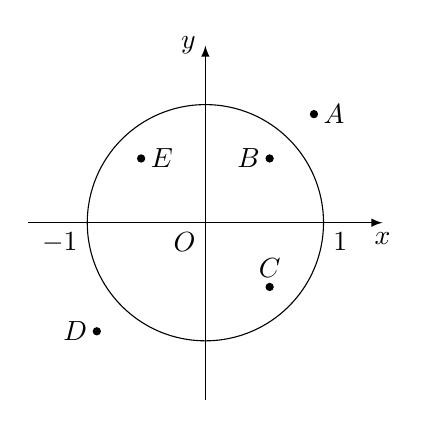
\begin{tikzpicture}[>=latex,scale = 1.5]
        \draw [->] (-1.5,0) -- (1.5,0) node [below] {$x$};
        \draw [->] (0,-1.5) -- (0,1.5) node [left] {$y$};
        \draw (0,0) node [below left] {$O$};
        \draw (0,0) circle (1);
        \filldraw (45:1.3) circle (0.03) node [right] {$A$};
        \filldraw (45:{1/1.3}) circle (0.03) node [left] {$B$};
        \filldraw (-45:{1/1.3}) circle (0.03) node [above] {$C$};
        \filldraw (135:{1/1.3}) circle (0.03) node [right] {$E$};
        \filldraw (225:1.3) circle (0.03) node [left] {$D$};
        \draw (1,0) node [below right] {$1$} (-1,0) node [below left] {$-1$};
    \end{tikzpicture}
\end{center}
\fourch{点$B$}{点$C$}{点$D$}{点$E$}
\item 把复数$a+b\mathrm{i}$($a,b\in R$)在复平间内的对应向量绕原点$O$顺时针方向旋转90°后, 所得向量对应的复数为\bracket{20}.
\fourch{$a-bi$}{$-a+bi$}{$b-ai$}{$-b+ai$}
\item 复平面内, 向量$\overrightarrow{OA}$, $\overrightarrow{OB}$分别对应于非零复数$z_1$, $z_2$, 若$\overrightarrow{OA}\perp \overrightarrow{OB}$, 则$\dfrac{z_2}{z_1}$一定是\bracket{20}.
\fourch{非负数}{纯虚数}{正实数}{非纯虚数}
\item 复数$z=(\sin 25^\circ +\mathrm{i}\cos 25^\circ)^3$的三角形式为\bracket{20}.
\fourch{$\sin 75^\circ +i\cos 75^\circ$}{$\cos 15^\circ +i\sin 15^\circ$}{$\cos 75^\circ +i\sin 75^\circ$}{$\cos 195^\circ +i\sin 195^\circ$}
\item $(1-\sqrt 3i)^2$的辐角主值为\bracket{20}.
\fourch{$\dfrac{10\pi }3$}{$\dfrac{7\pi }3$}{$\dfrac 43\pi$}{$\dfrac{\pi }3$}
\item (1)若$\alpha ,\beta ,\gamma$是一个三角形的三个内角, 则$(\cos \alpha +i\sin \alpha)(\cos \beta +i\sin \beta)(\cos \gamma +i\sin \gamma)=$\blank{50}.
(2)$(\cos 1^\circ +i\sin 1^\circ)(\cos 2^\circ +i\sin 2^\circ)(\cos 3^\circ +i\sin 3^\circ)\cdots (\cos 359^\circ +i\sin 359^\circ)=$\blank{50}.
(3)若$\dfrac{\sin A+i\cos A}{(\sin B+i\cos B)(\sin C+i\cos C)}$是纯虚数, 则$\triangle ABC$是\blank{50}三角形.
\item 计算下列各题:
(1)$\dfrac{{{[2(\cos 45^\circ +i\sin 45^\circ)]}^4}}{(\sin 80^\circ +i\cos 80^\circ)}=$\blank{50}.
(2)$\dfrac{{{(\sqrt 3+i)}^5}}{-1+\sqrt 3i}=$\blank{50}.
(3)$(1-\cos 60^{\circ }+i\sin 60^{\circ })=$\blank{50}.
(4)$(\cos 15^\circ -i\sin 15^\circ)^3+(\cos 15^\circ -i\sin 15^\circ)^{-3}=$\blank{50}.
\item (1)若$z=(\sqrt 3-i)^5$, 则$\arg z=$\blank{50}.
(2)若复数$z=7(\sin 140^\circ -\mathrm{i}\cos 140^\circ)$, 则$\arg (-\dfrac 1{z^2})=$\blank{50}.
(3)若$\arg z=\theta$, 则$\arg z^2=$\blank{50}.
(4)若$\arg z=\theta$, $\dfrac 43\pi \le \theta <2\pi$, 则$\arg z^3=$\blank{50}.
\item (1)复平面内, 将$1+\sqrt 3\mathrm{i}$所对应的向量绕原点按逆时针方向旋转$\theta$角, 所得向量对应的复数是$-2\mathrm{i}$, 则$\theta$的最小正值为\blank{50}.
(2)复平面内, 向量$\overrightarrow{AB}$对应的复数为$2+i$, 点$A$对应的复数为$-1$, 将$\overrightarrow{AB}$绕点$A$顺时针方向旋转90°后得到向量$\overrightarrow{AC}$, 则点$C$对应的复数为\blank{50}.
(3)若复数$z_1=\tan \theta -\mathrm{i}$, $z_2=\tan \theta +\mathrm{i}$($0<\theta <\dfrac{\pi }2$), 将$z_1$的对应向量顺时针旋转到$z_2$所对应的向量, 则所转过的最小正角等于\blank{50}.
(4)若复数$z_1\cdot z_2$满足$|z_1|=|z_2|=1$, $z_2-z_1=-1$, 则$\arg \dfrac{z_1}{z_2}=$\blank{50}.
(5)若$\arg (zi)=\theta$, $\theta \in (\dfrac{\pi }2,\pi)$, 则$\arg \overline z=$\blank{50}.
\item 若$\arg z_1=\alpha$, $\arg z_2=\beta$, 且$\alpha <\beta$, 则$\arg \dfrac{z_1}{z_2}$等于\bracket{20}.
\fourch{$\beta -\alpha$}{$\alpha -\beta$}{$2\pi +\alpha -\beta$}{$\pi +\beta -\alpha$}
\item 若$|z|=1$, $\arg z=\theta$($\theta \ne 0$), 则$\dfrac{z+\overline z}{1+{z^2}}$的辐角主值为\bracket{20}.
\fourch{$\dfrac{\theta }2$}{$\theta$}{$\pi -\theta$}{$2\pi -\theta$}
\item 若$z_1=1+\cos 2\theta +i\sin 2\theta$, $z_2=1-\cos 2\theta +i\sin \theta$, 则下列各式中必为定值的是\bracket{20}.
\fourch{$z_1\cdot z_2$}{$\dfrac{z_1}{z_2}$}{$|z_1|+|z_2|$}{$|z_1|^2+|z_2|^2$}
\item 若复数$-2+\mathrm{i}$和$3-\mathrm{i}$的辐角主值分别为$\alpha$和$\beta$, 则$\alpha +\beta$等于\bracket{20}.
\fourch{$\dfrac{3\pi }4$}{$\dfrac{5\pi }4$}{$\dfrac{7\pi }4$}{$\dfrac{11\pi }4$}
l00.复平面内, 已知点$P_1$, $P_2$分别对应于复数$3-2\mathrm{i}$, $7+4\mathrm{i}$, 线段$P_1P_2$绕点$P_1$按逆时针方向旋转$\dfrac 56\pi$到$P_1P_3$的位置, 则点$P_3$对应的复数为\bracket{20}.
\fourch{$2\sqrt 3+3\sqrt 3i$}{$2\sqrt 3-3\sqrt 3i$}{$-2\sqrt 3+3\sqrt 3i$}{$-2\sqrt 3-3\sqrt 3i$}
\item 复平面内, 点$P_1$的对应复数是$z_1=-2\sqrt 3+4\mathrm{i}$, 将向量$\overrightarrow{OP_1}$($O$为原点)旋转一个锐角$\theta$后得到新向量$\overrightarrow{OP_2}$, 且点$P_2$的对应复数是$z_2=\sqrt 3+5\mathrm{i}$, 则\bracket{20}.
\fourch{$\theta =60^{\circ }$, 且按逆时针旋转}{$\theta =60^{\circ }$, 且按顺时针旋转}{$\theta =30^{\circ }$, 且按逆时针旋转}{$\theta =30^{\circ }$, 且按顺时针旋转}
\item 已知$z_A=a+b\mathrm{i}$($a,b\in R$, 且$ab\ne 0$), 复平面内, 把$z_A$对应的向量$\overrightarrow{OA}$绕原点分别按逆、顺时针方向旋转$\dfrac{2\pi }3$, 得向量$\overrightarrow{OB}$, $\overrightarrow{OC}$, 则$\overrightarrow{OA}$, $\overrightarrow{OB}$, $\overrightarrow{OC}$所对应的复数之和等于\bracket{20}.
\fourch{$-a-bi$}{$-\dfrac 12+\dfrac{\sqrt 3}2i$}{$a-bi$}{0}
l03.若$\arg z\in [\dfrac{\pi }4,\dfrac{3\pi }4]$, 则$\arg (-\dfrac 1{zi})$的取值范围是\bracket{20}.
(4)$[\dfrac{3\pi }4,\dfrac{5\pi }4]$.						(B)$[\dfrac{5\pi }4,\dfrac{7\pi }4]$.
(C)$[\dfrac{\pi }4,\dfrac{7\pi }4]$.						(D)$[0,\dfrac{\pi }4]\cup [\dfrac{7\pi }4,2\pi)$.
\item 若数列$\{a_n\}$的通项公式为$a_n=(\cos \theta +i\sin \theta)^n$($\theta \ne 2k\pi$, $k\in \mathbf{Z}$), 则$\{a_n\}$\bracket{20}.
\fourch{成等差数列, 但不成等比数列}{成等比数列, 但不成等差数列}{成等差数列又成等比数列}{既不成等差数列也不成等比数列}
\item 若$(-\sqrt 3+i)^n\in \mathbf{R}^+$, 则最小的自然数$n$的值是\bracket{20}.
\fourch{6}{8}{10}{12}
\item 已知非纯虚数$z$满足$\arg z=\arg [(z+1)i]$, 则$z$在复平面内的对应点所表示的图形为\bracket{20}.
\fourch{\begin{tikzpicture}[>=latex,scale = 1.5]
    \draw [->] (-1.5,0) -- (0.5,0) node [below] {$x$};
    \draw [->] (0,-0.7) -- (0,0.7) node [left] {$y$};
    \draw (0,0) node [below left] {$O$};
    \draw (0,0) arc (0:180:0.5);
    \draw (-1,0) node [below] {$-1$};
    \filldraw [fill = white, draw = black] (0,0) circle (0.03);
    \filldraw [fill = white, draw = black] (-1,0) circle (0.03);
\end{tikzpicture}}{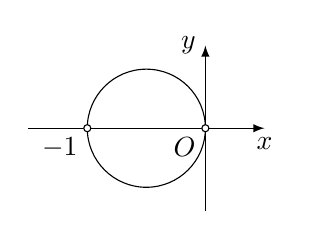
\begin{tikzpicture}[>=latex,scale = 1.5]
    \draw [->] (-1.5,0) -- (0.5,0) node [below] {$x$};
    \draw [->] (0,-0.7) -- (0,0.7) node [left] {$y$};
    \draw (0,0) node [below left] {$O$};
    \draw (-0.5,0) circle (0.5);
    \draw (-1,0) node [below left] {$-1$};
    \filldraw [fill = white, draw = black] (0,0) circle (0.03);
    \filldraw [fill = white, draw = black] (-1,0) circle (0.03);
\end{tikzpicture}}{\begin{tikzpicture}[>=latex,scale = 1.5]
    \draw [->] (-0.5,0) -- (1.5,0) node [below] {$x$};
    \draw [->] (0,-0.7) -- (0,0.7) node [left] {$y$};
    \draw (0,0) node [below left] {$O$};
    \draw (0,0) arc (180:0:0.5);
    \draw (1,0) node [below] {$1$};
    \filldraw [fill = white, draw = black] (0,0) circle (0.03);
    \filldraw [fill = white, draw = black] (1,0) circle (0.03);
\end{tikzpicture}}{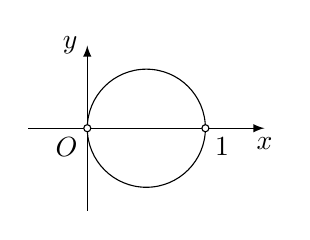
\begin{tikzpicture}[>=latex,scale = 1.5]
    \draw [->] (-0.5,0) -- (1.5,0) node [below] {$x$};
    \draw [->] (0,-0.7) -- (0,0.7) node [left] {$y$};
    \draw (0,0) node [below left] {$O$};
    \draw (0.5,0) circle (0.5);
    \draw (1,0) node [below right] {$1$};
    \filldraw [fill = white, draw = black] (0,0) circle (0.03);
    \filldraw [fill = white, draw = black] (1,0) circle (0.03);
\end{tikzpicture}}
\item 复平面内, 已知$\triangle ABC$的三个顶点分别对应于复数$z$, $\overline z$, $\dfrac 1z$, 且$|z|=3$, 点$A$的位置如图所示.
\begin{center}
    \begin{tikzpicture}[>=latex]
        \draw [->] (-1,0) -- (3,0) node [below] {$x$};
        \draw [->] (0,-1) -- (0,2) node [left] {$y$};
        \draw (0,0) node [below left] {$O$};
        \draw (0,0) -- (33:3) node [right] {$A$};
        \filldraw (33:1) circle (0.05) (33:2) circle (0.05); 
    \end{tikzpicture}
\end{center}

(1) 试在图上画出点$B,C$的大概位置;\\
(2) 求$\triangle ABC$面积的最大值.
\item (1)已知$|z_1|=3$, $|z_2|=5$, $|z_1-z_2|=7$, 求$\dfrac{z_1}{z_2}$.
(2)已知复数$z$满足$|z|=5$, 且$(3+4\mathrm{i})z$为纯虚数, 求$z$.
(3)若$|z|=1$, 求$|z^2-z+1|$的最大值和最小值.
(4)已知$z_1,z_2\in \mathbf{C}$, 且$|z_1|=|z_2|=1$, $z_1+z_2=\dfrac 45+\dfrac 35i$, 求$\tan (\arg z_1+\arg z_2)$.
(5)已知复数$z_1$和$z_2$满足$|z_1|=|z_2|=1$, 且$z_1-z_2=\dfrac 12-\dfrac 13\mathrm{i}$, 设$\theta$是$z_1\cdot z_2$的辐角, 求$\sin \theta$的值.
\item (1)已知复数$z_1,z_2,z_3$的辐角主值依次成公差为$\dfrac{2\pi }3$的等差数列, 且$|z_1|=|z_2|=|z_3|=1$, 求证: $z_1+z_2+z_3=0$.
(2)若复数$z_1,z_2,z_3$满足$z_1+z_2+z_3=0$, 且$|z_1|=|z_2|=|z_3|=1$, 求证: 复平面内以$z_1,z_2,z_3$所对应的点为顶点的三角形是内接于单位圆的正三角形.
(3)已知非零实数$x,y,z$满足了$x+y+z=0$, 复数$\alpha ,\beta ,\gamma$满足$|\alpha|=|\beta|=|\gamma|\ne 0$, 且$x\alpha +y\beta +z\gamma =0$, 求证: $\alpha =\beta =\gamma$.
\item (1)计算: $\arg (i+2)+\arg (i+3)$.
(2)若$\arg (-2-i)=\alpha$, $\arg (-3-i)=\beta$, 求$\alpha +\beta$.
\item 复平面内, 两点$A,B$分别对应于非零复数$\alpha ,\beta$, 试根据下列条件判断$\triangle OAB$的形状($O$为原点):
(1)$\alpha =\beta (\cos \theta +i\sin \theta)$($0<\theta <\pi$).	(2)$\alpha =\pm \beta i$.
(3)$\dfrac{\alpha }{\beta }=\pm \sqrt 3i$.							(4)$\dfrac{\alpha }{\beta }=\dfrac{1+\sqrt 3i}2$.
(5)$\dfrac{\alpha }{\beta }=1+i$.
\item (1)已知复数$z_1,z_2$满足$4z_1^2-2z_1z_2+z_2^2=0$, 且$|z_2|=4$, $z_1$, $z_2$, 0所对应的点分别为$A$, $B$, $O$, 求$\triangle AOB$的面积.
(2)复平面内, 点$A$, $B$分别对应于复数$\omega -z$和$\omega +z$, 其中$\omega =-\dfrac 12+\dfrac{\sqrt 3}2i$, 若$\triangle AOB$是以原点$O$为直角顶点的等腰直角三角形.求:
\textcircled{1} 复数$z$.							\textcircled{2} $\triangle AOB$的面积.
\item (1)已知等边三角形的两个顶点$A$, $B$对应的复数分别为$z_A=2+i$, $z_B=3+2i$, 求第三个顶点$C$所对应的复数.
(2)复平面内, 等边三角形的一个顶点在原点, 中心$P$所对应的复数是$1+\mathrm{i}$, 求其他两个顶点所对应的复数.
(3)复平而内, 矩形$OMNP$的相邻两边之比是$|OM|:|OP|=1:\sqrt 3$, 且点$O$, $M$的对应复数分别是0, $-1+2i$, 求点$N$对应的复数.
(4)已知等腰Rt$\triangle ABC$的斜边$AB$的两个端点的坐标分别为$A(-1,2)$, $B(2,3)$, 求顶点$C$的坐标.
(5)若等边$\triangle ABC$的一个顶点为$A(0,5)$, 中心$M$的坐标是$M(2,3)$, 求其他两个顶点$B$, $C$的坐标.
\item 已知复数$z_1=1+(2-\sqrt 3)\mathrm{i}$, $z_3=(2+\sqrt 3)+\mathrm{i}$, 又复数$z_1$, $z_2$, $z_3$, $z_4$在复平面内的对应点依逆时针方向排列足一个正方形的四个顶点.
(1)求$z_2$, $z_4$.
(2)求证: $z_2$, $z_4$, 0的对应点是一个等边三角形的三个顶点.
\item 复平面内, 已知$\triangle AOB$的顶点$A$, $B$所对应的复数$\alpha$, $\beta$满足$\beta +(1-\mathrm{i})\alpha =0$, 且$\triangle AOB$($O$为原点)面积的最大值和最小值分别是8和2, 求$|\alpha|$与$|\beta|$的取值范围.
\item (1)已知复数$z_1$, $z_2$, $z_3$满足$\dfrac{{z_2}-{z_1}}{{z_3}-{z_1}}=1+\sqrt 3i$, 试判断复平面内的$z_1$, $z_2$, $z_3$的对应点为顶点的三角形的形状, 并求其各内角的值.
(2)复平面内, 已知$A$, $B$, $C$三点对应的复数$z_1$, $z_2$, $z_3$满足$\dfrac{{z_2}-{z_1}}{{z_3}-{z_1}}=1+\dfrac 34\mathrm{i}$, 试求这个三角形三边长之比.
\item (1)—个三角形的底边$BC$的两端所表水的复数是$z_B=a$, $z_C=-a$, 顶点$A$的位置不定, 以两边$AB$, $AC$为腰, 分别以$B$, $C$为直角的顶点, 在$\triangle ABC$外作等腰直角三角形$ABD$, $ACE$, 求证: $DE$的中点$M$为定点,
(2)已知$B$是半圆$x^2+y^2=1$($y\ge 0$)上的动点, $A(2,0)$是$x$轴上的一个定点, 以$A$为直角顶点作等腰直角$\triangle ABC$(字母按顺时针排列), 求$|OC|$的最大值及其相应的点$B$的坐标($O$为坐标原点).
\item (1)复平面内, 已知Rt$\triangle ABC$的三个顶点$A$, $B$, $C$分别对应于复数$z$, $z^2$, $z^3$, 且$|z|=2$, $\angle BAC=90^{\circ }$, 求复数$z$.
(2)已知复数$z_1$满足$\arg z_1=\dfrac{5\pi }{12}$, $|z_1-z_0|=\sqrt 2$, $z_0-(1+i)z_1=0$.
\textcircled{1} 求$z_1$和$z_0$;
\textcircled{2} 求证: 在满足$|z_1-z_0|=\sqrt 2$条件的所有复数$z$中, $z_1$的辐角主值最小.
\item 已知复数$z=[\cos (\pi +\alpha)+i\sin (\pi +\alpha)]\cdot [\sin (\dfrac 32\pi +\beta)+i\cos (\dfrac 32\pi +\beta)]$, $0<\beta <\alpha <\dfrac{\pi }2$, 且$\sin (\alpha +\beta)=4\cos \alpha \sin \beta$, 求$\arg z$的最大值.
\item 已知$|z-1-\mathrm{i}|=2$, 求复数$z^2$虚部的取值范围.
\item 已知复数$z=x+yi$满足$|z+\dfrac 1z|=1$($x,y\in \mathbf{R}$).求证:
(1)$(x^2+y^2)^2+x^2-3y^2+1=0$.
(2)$k\pi +\dfrac{\pi }3\le \arg z\le k\pi +\dfrac{2\pi }3$($k\in \mathbf{Z}$).
(3)$\dfrac{\sqrt 5-1}2\le|z|\le \dfrac{\sqrt 5+1}2$.
\item 对$n\in \mathbf{N}$, $k\in \mathbf{N}$, 求证:
(1)$(\dfrac{1+i}{\sqrt 2})^n+(\dfrac{1-i}{\sqrt 2})^n=2\cos \dfrac{n\pi }4$.
(2)$(1+\cos \alpha +i\sin \alpha)^n=2^n\cos ^n(\dfrac{\alpha }2)(\cos \dfrac{n\alpha }2+i\sin \dfrac{n\alpha }2)$.
(3)$(\dfrac{1+i\tan \alpha }{1-i\tan \alpha })^n=\dfrac{1+i\tan n\alpha }{1-i\tan n\alpha }$.
(4)$(\dfrac{1-\cos \theta +i\sin \theta }{1-\cos \theta -i\sin \theta })^n=\cos n(\pi +\theta)-i\sin n(\pi +\theta)$($\theta \ne 2k\pi$).
\item (1)若$(1+\sqrt 3i)^n$是—个实数, 求自然数$n$的值.
(2)已知复数$z=\dfrac{{{(1+\mathrm{i})}^3}}{\sqrt 2{{(a+\mathrm{i})}^2}}$($a>0$)满足$|z|=\dfrac 12$.求:
\textcircled{1} $a$的值; 								\textcircled{2} 使$z^n$为实数的最小自然数$n$.
\item 已知数列$\{a_n\}$的通项$a_n=\dfrac 1{(1+\sqrt 3i)^n}$, 当$n$取1, 2, 3, …时, 依次得到的实数记为$b_1$, $b_2$, $b_3$, …, 求数列$\{b_n\}$的所有项之和.
\item (1)已知复数$z=\cos 20^\circ +\mathrm{i}\sin 20^\circ$, 求$|z-z^2+z^3-z^4+z^5-z^6+z^7-z^8+z^9-z^{10}|$.
(2)设$z=\cos 40^\circ +i\sin 40^\circ$, 求$|z+z^2+\cdots +z^{100}|$.
(3)已知$z=\cos \dfrac{2\pi }5+i\sin \dfrac{2\pi }5$, 求$(1+z^8)(1+z^4)(1+z^2)(1+z)$.
(4)已知$z=\cos \dfrac{\pi }3+i\sin \dfrac{\pi }3$, 求$|z+2z^2+3z^3+\cdots +12z^{12}|$.
\item 已知$z_n=(\dfrac{1+i}2)^n$($n\in \mathbf{N}$).
(1)记$a_n=|z_{n+1}|-|z_n|$($n\in \mathbf{N}$), 求数列$\{a_n\}$所有项之和.
(2)记$b_n=|z_{n+2}-z_n|$($n\in \mathbf{N}$), 求数列$\{b_n\}$所有项之和.
\item 设复数$z=\cos \theta +\mathrm{i}\sin \theta$($0<\theta <\pi$), $\omega =\dfrac{1-{{({\overline z})}^4}}{1+{z^4}}$, 且$|\omega|=\dfrac{\sqrt 3}3$, $\arg \omega <\dfrac{\pi }2$, 求$\theta$.
\item 已知复数$z=\cos \theta +i\sin \theta$($0<\theta <2\pi$), $\omega =\dfrac{1-{z^3}}{1-z}$.求:
(1)满足$|\omega|=1$的复数$z$.
(2)$\omega$的辐角(用$\theta$表示).
四、复数方程
【典型题型和解题技巧】
复数方程主要有以下几种类型:
1, —次方程$az=b$($a,b\in \mathbf{C}$, $a\ne 0$).
此类方程的解是$z=\dfrac ba$.
\item 解方程$3z+i=2iz+1$.
解  由已知, 得$(3-2i)z=1-i$, ∴$z=\dfrac{1-i}{3-2i}=\dfrac{(1-i)(3+2i)}{13}=\dfrac 5{13}-\dfrac 1{13}i$.
注意  关于$z$的一次方程, 若令$z=a+bi$($a,b\in \mathbf{R}$)也可获解, 但显然不妥.
\item 二次方程$az^2+bz+c=0$($a,b,c\in \mathbf{C}$, $a\ne 0$).
对于这类方程需强调两点:
韦达定理仍可沿用——若$\alpha$, $\beta$是上述方程的两根, 则$\begin{cases} \alpha +\beta =-\dfrac ba, \\ \alpha \beta =\dfrac ca, \end{cases}$反之亦真;
若$a$, $b$, $c$不全是实数, 则$\triangle =b^2-4ac$不能用来判断方程有无实根.
(1)二次方程$az^2+bz+c=0$($a,b,c\in \mathbf{C}$, $a\ne 0$), 这就是通常所说的``实系数—元二次方程.
解此类方程可分为两步:
第一步, 先算$\triangle =b^2-4ac$;
第二步, 若$\triangle \ge 0$, 则方程的解是$z=\dfrac{-b\pm \sqrt {\triangle }}{2a}$;
若$\triangle <0$, 则方程的解是$z=\dfrac{-b\pm \sqrt {-\triangle }i}{2a}$.
显然, 此类方程的$\triangle =b^2-4ac$可以用来判断此方程有无实根, 若方程有虚根, 则虚根一定``成对出现'', 即若$p+qi$($p\cdot q\in \mathbf{R}$)是上述方程的根, 则$p-qi$也是此方程的根.
\item 设$x$是模不为1的虚数, 记$y=x+\dfrac 1x$, 求满足$y^2+ay+1=0$的实数$a$的取值范围.
解  由题意可设$x=r(\cos \theta +i\sin \theta)$($r>0$, $r\ne 1$, $\theta \ne k\pi$),
则$y=x+\dfrac 1x=r(\cos \theta +i\sin \theta)+\dfrac 1r(\cos \theta -i\sin \theta)=(r+\dfrac 1r)\cos \theta +i(r-\dfrac 1r)\sin \theta$.
∵$\theta \ne k\pi$, $r>0$, 且$r\ne 1$, ∴$(r-\dfrac 1r)\sin \theta \ne 0$.
故$y$是虚数, 即方程$y^2+ay+1=0$有虚数根, ∴$\triangle =a^2-a<0$,
故实数$a$的取值范围是$-2<a<2$.
\item 已知关于$x$的实系数方程$z^2-2pz+q=0$($p\ne 0$)的两虚根$z_1$, $z_2$在复平面内的对应点为$F_1$, $F_2$, 求以$F_1$, $F_2$为两焦点, 且经过原点的椭圆的普通方程.
解  设$z_1=a+bi$($a,b\in \mathbf{R}$), 则$z_2=a-bi$.
由韦达定理, 得$\begin{cases} z_1+z_2=2a=2p, \\ z_1z_2=a^2+b^2=q. \end{cases}$
于是$a=p$, $|OF_1|=|OF_2|=\sqrt {a^2+b^2}=\sqrt q$(如图).显然, 椭圆的半短轴长$=|OM|=|a|=|p|$, 半焦距$=|b|$, 半长轴$=\sqrt {a^2+b^2}=\sqrt q$, 而椭圆的中心为$(a,0)$, 即$(p,0)$, 所以椭圆的普通方程为$\dfrac{{{(x-p)}^2}}{p^2}+\dfrac{y^2}q=1$.
\begin{center}
    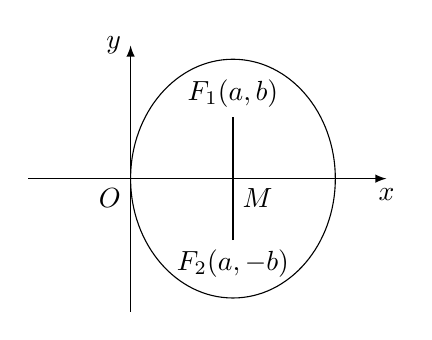
\begin{tikzpicture}[>=latex, scale = 1.3]
        \draw [->] (-1,0) -- (2.5,0) node [below] {$x$};
        \draw [->] (0,-1.3) -- (0,1.3) node [left] {$y$};
        \draw (0,0) node [below left] {$O$};
        \draw (1,0) ellipse (1 and {sqrt(1.36)});
        \draw (1,-0.6) node [below] {$F_2(a,-b)$} -- (1,0.6) node [above] {$F_1(a,b)$} (1,0) node [below right] {$M$};
    \end{tikzpicture}
\end{center}
(2)齐二次方程$az_1^2+bz_1z_2+cz_2^2=0$($a,b,c\in \mathbf{R}$, $a\ne 0$).此类方程称为关于$z_1$, $z_2$的齐二次方程, 在$z_2\ne 0$的前提下, 方程可变形为$a(\dfrac{z_1}{z_2})^2+b\cdot \dfrac{z_1}{z_2}+c=0$.若令$t=\dfrac{z_1}{z_2}$, 则有$at^2+bt+c=0$.
因此, 就实质而言, 它也是实系数的二次方程.
\item 若非零复数$z_1$, $z_2$在复平面内的对应点分别为$A$, $B$, 且满足$|z_2|=2$, $z_1^2-2z_1z_2+4z_2^2=0$.
(1)试判断$\triangle AOB$($O$为原点)的形状.	(2)求$\triangle AOB$的面积.
解  (1)由$z_1^2-2z_1z_2+4z_2^2=0$, 得$z_1=\dfrac{2z_2\pm 2\sqrt 3iz_2}2$, 即$z_1=(1\pm \sqrt 3i)z_2$,
即$z_1\text=2(\cos \dfrac{\pi }3\pm i\sin \dfrac{\pi }3)z_2$.由此得$\triangle AOB$是直角三舟形, 且$\angle AOB=60^{\circ }$.
(2)$S_{\triangle AOB}=\dfrac 12|AO|\cdot|BO|\sin \dfrac{\pi }3=\dfrac{\sqrt 3}4\cdot 2\cdot|BO|^2=2\sqrt 3$.
(3)二次方程$az^2+bz+c=0$($a$, $b$, $c$不全为实数, $a\ne 0$).
此类方程布些超过教科书的要求, 它的解法可按以下步骤进行:
先计算$\triangle =b^2-4ac$, 再把$\triangle$化成一个复数$u$的平方, 即$\triangle =u^2$,
然后用公式$z=\dfrac{-b\pm u}{2a}$.
\item 解方程$x^2-(3-2i)x+5-5i=0$.
解  ∵$\triangle =(3-2i)^2-4(5-5i)=-15+8i=(1+4i)^2$,
∴$x=\dfrac{3-2i\pm (1+4i)}2$.故$x_1=2+i$, $x_2=1-3i$.
\item —元高次方程.
本单元出现的一元高次方程的系数均为实数, 即$a_nx^n+a_{n-1}x^{n-1}+\cdots +a_1x+a_0=0$, 其中$a_k\in \mathbf{R}$($k=0,1,2,3,\cdots n$).
解实系数的高次方程主要有下面两种方法.
(1)分解因式法.
\item 解方程$x^3+8=0$.
解  原方程即为$(x+2)(x^2-2x+4)=0$.
由$x+2=0$, 得$x=-2$.由$x^2-2x+4=0$, 得$x=1\pm \sqrt 3i$.
∴原方程的解为$x_1=-2$, $x_2=1+\sqrt 3i$, $x_3=1-\sqrt 3i$.
(2)公式法.
所谓公式法, 即对于``$n$次方程''$z^n=a$(常数$a\in \mathbf{C}$), 可利用公式求解.
先将$a$化成三角形式, 即$a=r(\cos \theta +i\sin \theta)$($r>0$).
再用公式$z=\sqrt[n]r(\cos \dfrac{2k\pi +\theta }n+i\sin \dfrac{2k\pi +\theta }n)$($k=0,1,2,\cdots n-1$).
\item 解方程$(1+z)^n-(1-z)^n=0$.
解  由已知, 得$(1+z)^n=(1-z)^n$, 显然$(1-z)^n\ne 0$, 故有$(\dfrac{1+z}{1-z})^n=1$.
∴$\dfrac{1+z}{1-z}=\cos \dfrac{2k\pi }n+i\sin \dfrac{2k\pi }n$($k=0,1,2,\cdots n-1$).由合分比定理得
$z=\dfrac{\cos \dfrac{2k\pi }n+i\sin \dfrac{2k\pi }n-1}{\cos \dfrac{2k\pi }n+i\sin \dfrac{2k\pi }n+1}=\dfrac{\sin \dfrac{k\pi }n(-\sin \dfrac{k\pi }n+i\cos \dfrac{k\pi }n)}{\cos \dfrac{k\pi }n(\cos \dfrac{k\pi }n+i\sin \dfrac{k\pi }n)}=\tan \dfrac{k\pi }n\cdot \dfrac{(\cos \dfrac{k\pi }n+i\sin \dfrac{k\pi }n)i}{(\cos \dfrac{k\pi }n+i\sin \dfrac{k\pi }n)}$
 $=-i\tan \dfrac{k\pi }n$($n=0,1,2,\cdots ,n-1$).
\item 方程$f(z,\overline z,|z|)=0$.
这是一类比较特殊的方程, 方程中含有$z$, $\overline z$和$|z|$.解此类方程通常有以下两种方法.
(1)代数式法.
所谓代数式法, 即令$z=x+yi$($x,y\in \mathbf{R}$)代入方程求解.
\item 解方程$(\overline z)^2=z$.
解  令$z=x+yi$($x,y\in \mathbf{R}$), 则有$(x-yi)^2=x+yi$,
即$x^2-y^2-2xyi=x+yi$, 于是$\begin{cases} x^2-y^2=x, \\ -2xy=y. \end{cases}$
若$y=0$, 则$x^2=x$, 得$x=0$或$x=1$, ∴$z_1=0$, $z_2=1$.
若$y\ne 0$, 则$x=-\dfrac 12$, $y=\pm \dfrac{\sqrt 3}2$, ∴$z_3=-\dfrac 12+\dfrac{\sqrt 3}2i$, $z_4=-\dfrac 12-\dfrac{\sqrt 3}2i$.
∴方程的解为0, 1, $-\dfrac 12\pm \dfrac{\sqrt 3}2i$.
(2)定性法.
有一类方程, 可以通过初步观察, 对方程的根先``定性'', 从而为求解带来一定的方便.
\item 解方程$z^2-4|z|+3=0$.
解  由已知, $z^2=-3+4|z|$, 故$z^2$必是实数, 因此, $z$是实数或纯虚数.
(1)$z$是实数时, 原方程即为$|z|^2-4|z|+3=0$, ∴$(|z|-1)(|z|-3)=0$,
于是得$z=\pm 1$或$z=\pm 3$.
(2)$z$是纯虚数时, 可令$z=ti$($t\in \mathbf{R}$, $t\ne 0$), 则原方程即为$(ti)^2-4|ti|+3=0$, 即$-t^2-4|t|+3=0$, 即$|t|^2+4|t|-3=0$, ∴$|t|=-2+\sqrt 7$,
故$z=\pm (-2+\sqrt 7)i$.方程的解为$\pm 1$, $\pm 3$, $\pm (2-\sqrt 7)i$
【训练题】
\item 若$z\in \mathbf{C}$, 则方程$|z|^2-|z|=0$解的个数是\bracket{20}.
\fourch{2}{3}{5}{无穷多}
\item 方程$z^2=\overline z$的解的个数是\bracket{20}.
\fourch{2}{3}{4}{5}
\item 二次方程$x^2-2xi-5=0$的根的情况是\bracket{20}.
\fourch{有两个不等的实根}{有一个实根和一个虚根}{有一对共轭的虚根}{有两个不共轭的虚根}
\item 满足$z+|\overline z|=2+\mathrm{i}$的复数$z$等于\bracket{20}.
\fourch{$-\dfrac 34+i$}{$\dfrac 34-i$}{$-\dfrac 34-i$}{$\dfrac 34+i$}
\item 若关于$x$的方程$x^2+x+p=0$的两个虚根$\alpha$, $\beta$满足$|\alpha -\beta|=3$, 则实数$p$的值为\bracket{20}.
\fourch{-2}{$-\dfrac 12$}{$\dfrac 52$}{1}
\item 若$a>1$, $\alpha$, $\beta$是关于$x$的方程$x^2+2x+a=0$的两根, 则$|\alpha|+|\beta|$的值为\bracket{20}.
\fourch{2}{$2\sqrt a$}{$2\sqrt {a-1}$}{$2\sqrt {1-a}$}
\item (1)若关于$x$的实系数二次方程$x^2+ax+b=0$的一个根是$2+i$, 则$a=$\blank{50}, $b=$\blank{50}.
(2)若实系数的一元二次方程的一个根是$\dfrac 13-\dfrac{4\sqrt 5}3i$, 则这个方程为\blank{50}.
\item 1的5次方根的五个复数的辐角主值之和是\bracket{20}.
\fourch{$2\pi$}{$4\pi$}{$6\pi$}{$8\pi$}
\item 若$\omega$是$x^5-1=0$的一个虚根, 则$\omega (1+\omega)(1+\omega ^2)$的值是\bracket{20}.
\fourch{1}{-1}{$i$}{$-\dfrac 12+\dfrac{\sqrt 3}2i$}
\item 复平面内, 两点$M$, $N$所对应的非零复数是$\alpha$, $\beta$($O$是原点).
(1)若$\alpha ^2+\beta ^2=0$, 则$\triangle OMN$是\blank{50}三角形.
(2)若$2\alpha ^2-2\alpha \beta +\beta ^2=0$, 则$\triangle OMN$是\blank{50}三角形.
\item 在复数范围内解方程:
(1)$z\cdot \overline z-3i\overline z=1+3i$.				(2)$z^2-5|z|+6=0$.
(3)$2z+|z|=2+6i$.					(4)$z|z|+az+i=0$($a\ge 0$).
(5)$|z|^2-2zi+2a(1+i)=0$($a\in \mathbf{R}$).
\item (1)已知关于$x$的方程$x^2+(k+2i)x+2+ki=0$有一个实根, 求实数$k$的值.
(2)已知关于$x$的方程$x^2-ix-m+4ni=0$有实根, 求点$(m,n)$应满足的方程.
(3)已知关于$x$的方程$x^2-zx+4+3\mathrm{i}=0$有实根, 求复数$z$的模的最小值和此时的$z$值.
\item (1)已知方程$x^2+ix+6=2i+5x$有一个实数解, 试在复数范围内解此方程.
(2)已知关于$x$的方程$x^2+2px+1=0$的两根$\alpha$, $\beta$在复平面内的对应点和原点恰是一个等边三角形的三个顶点, 求实数$p$的值.
(3)已知$p,q\in \mathbf{R}$, 方程$x^2+px+q=0$有两虚根$\alpha$, $\beta$, 方程$x^2-px+q=0$有两虚根$\alpha ^2$, $\beta ^2$, 求$\alpha$, $\beta$, $p$, $q$的值.
(4)已知$a$, $b$是实数, 关于$x$的方程$x^2+(2a-b\mathrm{i})x+a-b\mathrm{i}=0$的两个非零复数根的辐角分別为$\dfrac{2\pi }3$及$\pi$, 求$a$, $b$的值.
\item (1)求$5+12i$的平方根.
(2)解方程: \textcircled{1} $z^2-i=0$.				\textcircled{2} $z^2-2zi-5=0$.
\item 复平面内, 已知非零复数$z_1$, $z_2$对应于点$A$和$B$, 复数$z_1-a$与$z_1+a$所对应的两个向量相互垂直且模不相等, 又$z_1^2-4z_1z_2+6z_2^2=0$.
(1)求$z_1$与$z_2$的模.
(2)$O$为复平面上的坐标原点, 求$\triangle AOB$的面积.
\item 非零复数$\alpha$, $\beta$分别对应于点$A$, $B$($O$是原点), 已知$4\alpha ^2-2\alpha \beta +\beta ^2=0$.
(1)求证: $\triangle AOB$是直角三角形.
(2)若$|\alpha|=1$, 求$\triangle AOB$的面积.
(3)若$|\alpha|=t>0$, 求$|\beta|^2-\alpha \overline \beta -\overline \alpha \beta$的值.
\item 设$\alpha$, $\beta$是实系数一元二次方程$ax^2+bx+c=0$的两根, $\alpha$为虚数, 而$\dfrac{{{\alpha }^2}}{\beta }$为实数, 求复数$\dfrac{\alpha }{\beta }$的值.
\item 已知: $x+\dfrac 1x=2\cos \varphi$.求证:
(1)$x=\cos \varphi \pm i\sin \varphi$.
(2)$x^n+\dfrac 1{x^n}=2\cos n\varphi$($n\in \mathbf{N}$).
\item (1)要使关于$x$的方程$(1-i)x^2+2mix-(1+i)=0$有实根, 求实数$m$的值.
(2)若关于$x$的实系数方程$2x^2+3ax+a^2-a=0$至少布一个模为1的根, 求实数$a$的值.
(3)若关于$x$的方程$x^2+(2+i)x+4mn+(2m-n)i=0$($m,n\in \mathbf{R}$)有实根, 求点$(m,n)$的轨迹方程.
(4)已知$\alpha$, $\beta$是方程$x^2-2x+2=0$的两根, $p$, $q$是关于$x$的方程$x^2+2mx-1=0$($m\in \mathbf{R}$)的两根, 且$\alpha$, $\beta$, $p$, $q$在复平面内的对应点共圆, 求$m$的值.
(5)已知关于$x$的方程$3x^2-6(m-1)x+m^2+1=0$的两根$x_1$, $x_2$满足$|x_1|+|x_2|=2$, 求实数$m$的值.
\item (1)实系数方程$x^4-4x^3+9x^2-ax+b=0$的一个根是$1+i$, 求$a$, $b$的值, 并解此方程.
(2)已知关于$x$的实系数方程$x^4+ax^3+bx^2+cx+d=0$有一个纯虚根, 求证: $a^2d+c^2-abc=0$.
(3)已知模为2, 辐角为$\dfrac{\pi }6$的复数是方程$x^5+a=0$的一个根, 求$a$.
(4)已知复数$z=\dfrac 12+\dfrac{\sqrt 3}2i$满足$z^n=\overline z$, 求整数$n$的一般形式.
\item 利用复数乘法、除法的几何意义, 求证:
(1)$\arctan 1+\arctan 2+\arctan 3=\pi$.
(2)$\arcsin \dfrac{\sqrt {10}}{10}+\arccos \dfrac{7\sqrt 2}{10}+\arctan \dfrac 7{31}+arc\cot 10=\dfrac{\pi }4$.
(3)$\arctan (3+2\sqrt 2)-\arctan \dfrac{\sqrt 2}2=\dfrac{\pi }4$.
(4)$\arctan \dfrac 17+2\arcsin \dfrac 1{\sqrt {10}}=\dfrac{\pi }4$.
\item (1)复平面内, 已知动点$A$, $B$所对应的复数$z_1$, $z_2$的一个辐角为定值$\theta$和$-\theta$($0<\theta <\dfrac{\pi }2$), 且$\triangle AOB$的面积为定值$S$($O$为坐标原点〉, 求$\triangle AOB$的重心$M$所对应复数$z$的模的最小值.
(2)复数$z_1$, $z_2$, $z_3$的辐角主值分别为$\alpha$, $\beta$, $\gamma$, 模分别为1, $k$和$2-k$, 且$z_1+z_2+z_3=0$, 求$k$, 使$\cos (\beta -\alpha)$分别取到最大值和最小值, 并求出大值和最小值.
\item 已知复数$z=\cos \theta +\mathrm{i}\sin \theta$.
(1)当实数$k$和$\theta$分别为何值时, $z^3+k\overline z^3$是纯虚数?
(2)求$|z^3+k\overline z^3|$的最大值与最小值.
\item (1)已知复数$z_1$, $z_2$, $z_3$满足$|z_1|=|z_2|=|z_3|=1$, 求证: $|z_1z_2+z_2z_3+z_3z_1|=|z_1+z_2+z_3|$.
(2)已知复数$\alpha$, $\beta$, $\gamma$满足$|\alpha|=|\beta|=|\gamma|\ne 0$, 求证: $\dfrac{(\alpha +\beta)(\beta +\gamma)(\gamma +\alpha)}{\alpha \beta \gamma }$是实数.
\item 设$A$, $B$, $C$分别是复数$z_1$, $z_2$, $z_3$($z_1$, $z_2$, $z_3$互不相等)在复平面内所对应的点, 求证: $\triangle ABC$为等边三角形的充要条件是$z_1^2+z_2^2+z_3^2=z_1z_2+z_2z_3+z_3z_1$.
\item 利用复数知识证明: $\cos 3\alpha =4\cos ^3\alpha -3\cos \alpha$, $\sin 3\alpha =3\sin \alpha -4\sin ^3\alpha$.
\item (1)求证: $\cos \dfrac{\pi }{2n+1}+\cos \dfrac{3\pi }{2n+1}+\cos \dfrac{5\pi }{2n+1}+\cdots +\cos \dfrac{2n-1}{2n+1}\pi =\dfrac 12$($n\in \mathbf{N}$).
(2)已知$\cos \alpha +\cos \beta +\cos \gamma =0$, $\sin \alpha +\sin \beta +\sin \gamma =0$.求证:
\textcircled{1} $\cos 3\alpha +\cos 3\beta +\cos 3\gamma =3\cos (\alpha +\beta +\gamma)$, $\sin 3\alpha +\sin 3\beta +\sin 3\gamma =3\sin (\alpha +\beta +\gamma)$;
\textcircled{2} $\cos 3k\alpha =\cos 3k\beta =\cos 3k\gamma =\cos k(\alpha +\beta +\gamma)$,
$\sin 3k\alpha =\sin 3k\beta =\sin 3k\gamma =\sin k(\alpha +\beta +\gamma)$($k\in \mathbf{N}$).
\item (1)若$|z|=1$, 求复数$u=3z^2+\dfrac 1{z^2}$在复平面内的对应点的轨迹.
(2)求复数$z=\dfrac 1{1-bi}$($b\in \mathbf{R}$且$b\ne 0$)在复平面内对应点的轨迹方程.
(3)复平面内, 若复数$z$对应的点在连接复数$2+\mathrm{i}$和$2-\mathrm{i}$对应点的线段上移动, 求$z^2$对应点的轨迹方程.
\item 根据条件, 求复数$z+\dfrac 1z$在复平面内的对应点轨迹的普通方程:
(1)$|z|=1$.
(2)$|z|=r$($r>0$, $r\ne 1$).
(3)$|z|\ne 0$, 且$\arg z=\theta$.
\item (1)在等腰Rt$\triangle ABC$中, 已知$\angle C=90^{\circ }$, $|AC|=a$.若点$A$在$x$轴上移动, 点$B$在抛物线上移动, 且点$A$, $B$, $C$按逆时针方向排列, 求顶点$C$的轨迹方程.
(2)设$P$是抛物线$y=x^2$上任意一点, 以线段$OP$为边, 按逆时针方向作正方形$OPQR$(如图), 利用复数知识求点$R$的轨迹方程.
\begin{center}
    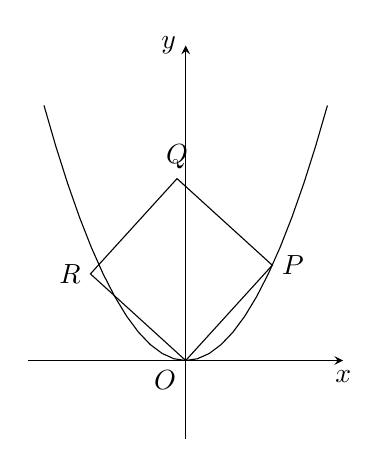
\begin{tikzpicture}[>=stealth]
        \draw [->] (-2,0) -- (2,0) node [below] {$x$};
        \draw [->] (0,-1) -- (0,4) node [left] {$y$};
        \draw (0,0) node [below left] {$O$} coordinate (O);
        \draw [domain = -1.8:1.8] plot (\x,{\x*\x});
        \draw (1.1,1.21) node [right] {$P$} coordinate (P);
        \draw ($(O)!1!90:(P)$) node [left] {$R$} coordinate (R);
        \draw ($(O)!{sqrt(2)}!45:(P)$) node [above] {$Q$} coordinate (Q);
        \draw (O) -- (P) -- (Q) -- (R) -- cycle;
    \end{tikzpicture}
\end{center}
\item 一动点从原点出发, 开始沿$x$轴的正半轴运动, 每运动一个长度单位, 就向左转$\theta$角, 求此动点运动$n$个长度单位时与原点的距离.
\item (1)复平面内, 复数$\alpha$的对应点在连接$1+\mathrm{i}$和$1-\mathrm{i}$的对应两点的线段上运动, 复数$\beta$的对应点在以原点为圆心, 半径为1的圆周上运动, 试求:
\textcircled{1} 复数$\alpha +\beta$的对应点运动范围的面积; 		\textcircled{2} 复数$\alpha \beta$的对应点运动范围的面积.
(2)已知半径为1的定圆$O$的内接正$n$边形的顶点为$P_k$($k=1,2,\cdots n$), $P$为该圆周上任意一点, 求证: $|PP_1|^2+|PP_2|^2+\cdots +|PP_n|^2$为一定值.


\end{enumerate}
\end{document}